This chapter continues looking at the case where the MDP models are
large state space. In the previous chapter we looked at
approximating the value function. In this chapter we will consider
learning directly a policy and optimizing it.

\section{Problem Setting}

To describe the problem formally, we shall make an assumption about the policy structure and the optimization objective, as follows. 
% We will assume that each state $\state$ has an encoding
% $\phi(\state)\in \mathbb{R}^{d_1}$. 
The policy will have a
parametrization $\theta\in \mathbb{R}^{d}$, and we denote by 
$\policy(\action|\state,\theta)$ the probability of
selecting action $\action$ when observing state $\state$, and having a policy parametrization
$\theta$. 

For technical ease, we consider the stochastic shortest path objective described in Chapter \ref{chapter:episodic}:
\[\Value^\policy(\state) = \mathbb E^{\pi }\left[\left.\sum\limits_{\ttime = 0}^\termtime {{\reward_\ttime}} \right|\state_0 = \state\right],\]
where $\termtime$ is the termination time, which we will assume to bounded with probability one, i.e., Assumption \ref{ass:finite_termination_prob} holds.
We are given a distribution over the initial state of the MDP, $\initdist(\state_0)$, and define $J(\theta) \triangleq \mathbb{E}\left[ \Value^\policy(\state_0)\right] = \initdist^\top \Value^\policy$ to be the expected value of the policy (where the expectation is with respect to $\initdist$).

The optimization problem we consider is:
\begin{equation}\label{eq:policy_opt}
\theta^* = \arg\max_\theta J(\theta).
\end{equation}

% where $J(\theta) \triangleq \Value^\policy(\state_0)$ is the
% expected return of the policy $\policy(\cdot|\cdot,\theta)$ from the
% initial state $\state_0$.
%
This maximization problem can be solved in multiple ways. We will
mainly explore gradient based methods.

In the setting that the MDP is not known, we shall assume that we are allowed to simulate `rollouts' from a given policy, $\state_0,\action_0,\reward_0,\dots,\state_\termtime, \action_\termtime, \reward_\termtime$, where $\state_0 \sim \initdist$, $\action_\ttime\sim \policy(\cdot|\state_\ttime,\theta)$, and $\state_{\ttime+1} \sim \transitionkernel (\cdot | \state_\ttime, \action_\ttime)$. We shall devise algorithms that use such rollouts to modify the policy parameters $\theta$ in a way that increases $J(\theta)$.

\section{Policy Representations}
We start with a few examples on how to parameterize the policy.
\paragraph{Log linear policy} We will assume a feature encoding
of the state and action pairs, i.e., $\phi(\state,\action)\in \mathbb{R}^{d}$. Given the parameter $\theta$, the linear part will compute $\xi(\state,\action)=\phi(\state,\action)^\top \theta$. Given the values of $\xi(\state,\action)$ for each $\action\in \Actions$, the policy selects action $\action$ with probability proportional to
$e^{\xi(\state,\action)}$. Namely,
\[
\policy(\action|\state,\theta)=
\frac{e^{\xi(\state,\action)}}{\sum_{b\in
\Actions}e^{\xi(\state,b)}}
\]
Note that this is essentially a soft-max selection over $\xi(\state,\action)$.

\paragraph{Gaussian linear policy} This policy representation applies when the action
space is a real number, i.e., $\Actions=\mathbb{R}$. The encoding of states is $\phi(\state)\in \mathbb{R}^{d}$. Given a state $\state$,
we compute $\xi(\state)=\phi(\state)^\top\theta$. We select an
action $\action$ from the normal distribution with mean
$\xi(\state)$ and variance $\sigma^2$, that is, $\mathcal{N}(\xi(\state),\sigma^2)$ (the Gaussian policy has an additional parameter $\sigma$). For an action space with dimension larger than 1, we can consider such a policy with a different parameter vector $\theta$ for every dimension.

\paragraph{Non-linear policy} Note that in both the log linear and Gaussian linear policies above, the dependence of $\xi$ on $\theta$ was linear. It is straightforward to extend these policies such that $\xi$ depends on $\theta$ in a more expressive and non-linear manner. A popular parametrization is a feed-forward neural network, also called a multi-layered perceptron (MLP). An MLP with $d$ inputs, 2 hidden layers of sizes $h_1$, $h_2$, and $k$ outputs has parameters $\theta_0 \in \mathbb{R}^{d \times h_1}$, $\theta_1 \in \mathbb{R}^{h_1 \times h_2}$, $\theta_2 \in \mathbb{R}^{h_2 \times k}$. The MLP computes $\xi\in \mathbb{R}^{k}$ as follows:
\begin{equation*}
    \xi(\state) = \theta_2^T f_{nl}\left(\theta_1^T\left( f_{nl}\left(\theta_0^T \phi\left(\state \right)\right)\right)\right) \in \mathbb{R}^{k},
\end{equation*}
where $f_{nl}$ is some non-linear function that is applied element-wise to each component of a vector, for example the Rectified Linear Unit (ReLU) defined as $\text{ReLU}(x) = \max(0, x)$. Once $\xi$ is computed, selecting an
action proceeds similarly as above, e.g., by sampling from the normal distribution with mean
$\xi(\state)$ and variance $\sigma^2$.

\paragraph{Simplex policy} This policy representation will be used mostly for pedagogical reasons, and can express any Markov stochastic policy. For a finite state and action space, let $\theta \in [0,\infty)^{\States \times \Actions}$, and denote $\theta_{\state,\action}$ the parameter corresponding to state $\state$ and action $\action$. We define $\policy(\action|\state,\theta) = \frac{\theta_{\state,\action}}{\sum_{\action'} \theta_{\state,\action'}}$. Clearly, any Markov policy $\tilde{\policy}$ can be represented by setting $\theta_{\state,\action} = \tilde{\policy}(\action|\state)$.

\section{The Policy Performance Difference Lemma}

Considering the optimization problem \eqref{eq:policy_opt}, an important question is how a change in the parameters $\theta$, which induces a change in the policy $\policy$, relates to a change in the performance criterion $J(\theta)$. We shall derive a fundamental result known as the performance difference lemma.

Let $\transitionkernel^{\policy}(\state' | \state)$ denote the state transitions in the Markov chain induced by policy $\policy$ (following Section \ref{sec:ssp-bellman}, we only consider transitions between non-goal states). Let us define the visitation frequencies $\discdist^{\policy}(\state) = \sum_{t=0}^\infty \Pr(\state_t = \state | \initdist, \policy)$. We first establish the following result.
\begin{proposition}\label{prop:visitation_freq}
    We have that $\discdist^{\policy} = \initdist + \discdist^{\policy} \transitionkernel^{\policy}$, and therefore $\discdist^{\policy} = \initdist (I - \transitionkernel^{\policy})^{-1}$.
\end{proposition}
\begin{proof}
We have,
\begin{equation*}
\begin{split}
        \discdist^{\policy}(\state) &= \initdist(\state) + \sum_{t=1}^\infty \Pr(\state_t = \state | \initdist, \policy) \\
        &= \initdist(\state) + \sum_{t=1}^\infty \sum_{\state'} \Pr(\state_{t-1} = \state' | \initdist, \policy) \transitionkernel^{\policy}(\state | \state')\\
       &= \initdist(\state) +  \sum_{\state'} \transitionkernel^{\policy}(\state | \state') \sum_{t=1}^\infty \Pr(\state_{t-1} = \state' | \initdist, \policy) \\
        &= \initdist(\state) + \sum_{\state'} \discdist^{\policy}(\state')\transitionkernel^{\policy}(\state | \state').
\end{split}
\end{equation*}
Writing the result in matrix notation gives the first result. For the second result, Proposition \ref{prop:bellman_FP_ssp} showed that $(I - \transitionkernel^{\policy})$ is invertible. 
\end{proof}

To deal with large state spaces, as we did in previous chapters, we will want to use sampling to approximate quantities that depend on all states. Note that expectations over the state visitation frequencies can be approximated by sampling from policy rollouts.
\begin{proposition}\label{prop:rollout_sampling}
    Consider a random rollout from the policy $\state_0,\action_0,\reward_0,\dots,\state_\termtime, \action_\termtime, \reward_\termtime$, where $\state_0 \sim \initdist$, $\action_\ttime\sim \policy(\cdot|\state_\ttime,\theta)$, $\state_{\ttime+1} \sim \transitionkernel (\cdot | \state_\ttime, \action_\ttime)$, and $\termtime$ is the termination time. For some function of states $g(\state)$, we have that:
    \begin{equation*}
        \sum_{\state} \discdist^{\policy}(\state) g(\state) = \mathbb{E}^{\policy}\left[ \sum_{\ttime=0}^\tau g(\state_\ttime)\right].
    \end{equation*}
\end{proposition}
\begin{proof}
    We have
    \begin{equation*}
        \begin{split}
            \mathbb{E}^{\policy}\left[ \sum_{\ttime=0}^\tau g(\state_\ttime)\right] &= \mathbb{E}^{\policy}\left[ \sum_{\ttime=0}^\tau \sum_{\state} \IND(\state_\ttime = \state)g(\state_\ttime)\right] \\
            &= \sum_{\state}\mathbb{E}^{\policy}\left[\sum_{\ttime=0}^\tau \IND(\state_\ttime = \state)g(\state_\ttime)\right] \\
            &= \sum_{\state}\mathbb{E}^{\policy}\left[\sum_{\ttime=0}^\tau \IND(\state_\ttime = \state)g(\state)\right] \\
            &= \sum_{\state}g(\state)\mathbb{E}^{\policy}\left[\sum_{\ttime=0}^\tau \IND(\state_\ttime = \state)\right] \\
            &= \sum_{\state}g(\state)\discdist^{\policy}(\state) ,
        \end{split}
    \end{equation*}
where $\IND[\cdot]$ is the indicator function.
\end{proof}

We now state the performance difference lemma.
\begin{lemma}\label{lemma:perf_diff}
    For any two policies, $\policy$ and $\policy'$, corresponding to parameters $\theta$ and $\theta'$, we have
    \begin{equation}\label{eq:policy_perf_diff}
        J(\theta') - J(\theta)= \sum_{\state} \discdist^{\policy'}(\state) \sum_\action \policy'(\action|\state)\left( \QValue^{\policy}(\state,\action) - \Value^{\policy}(\state)\right).
    \end{equation}
\end{lemma}
\begin{proof}
    We have that $\Value^{\policy'} = (I - \transitionkernel^{\policy'})^{-1}\reward$, and therefore
    \begin{equation*}
    \begin{split}
        \Value^{\policy'} - \Value^\policy &= (I - \transitionkernel^{\policy'})^{-1}\reward - (I - \transitionkernel^{\policy'})^{-1} (I - \transitionkernel^{\policy'}) \Value^\policy \\
        &=(I - \transitionkernel^{\policy'})^{-1} \left(\reward +\transitionkernel^{\policy'}\Value^\policy - \Value^\policy \right).
    \end{split}
    \end{equation*}
    Multiplying both sides by $\initdist$, and by Proposition \ref{prop:visitation_freq} $\discdist^{\policy'}=\initdist (I - \transitionkernel^{\policy'})^{-1}$, this gives
    \begin{equation*}
        J(\theta') - J(\theta) = \discdist^{\policy'}\left(\reward +\transitionkernel^{\policy'}\Value^\policy - \Value^\policy \right).
    \end{equation*}
    Finally, note that $\sum_\action \policy'(\action|\state) \QValue^{\policy}(\state,\action) = \reward(\state) + \sum_{\state'}\transitionkernel^{\policy'}(\state'|\state)\Value^{\policy}(\state')$.
\end{proof}

Given some policy $\policy(\action|\state)$, an improved policy $\policy'(\action|\state)$ must satisfy that the right hand side of Eq.~\ref{eq:policy_perf_diff} is positive.
Let us try to intuitively understand this criterion. First, consider the simplex policy parametrization above, which can express any Markov policy.  Consider the policy iteration update $\policy'(\state) = \argmax_{\action} \QValue^{\policy}(\state,\action)$. Substituting in the right hand side of Eq.~\ref{eq:policy_perf_diff} yields a non-negative value for every $\state$, and therefore an improved policy as expected.

For some policy parametrizations, however, the terms in the sum in Eq.~\ref{eq:policy_perf_diff} cannot be made positive for all $\state$. To obtain policy improvement, the terms need to be balanced such that a positive sum is obtained. This is not straightforward for two reasons. First, for large state spaces, it is not tractable to compute the sum over $\state$, and sampling must be used to approximate this sum. However, straightforward sampling of states from a fixed policy will not work, as the weights in the sum, $\discdist^{\policy'}(\state)$, \textit{depend on the policy $\policy'$}! 
The basic insight is that when we modify $\policy$, we directly influence the action distribution, but we also indirectly change the state distribution, which influences the expected reward.

The following example shows that indeed, balancing the sum with respect to weights that correspond to \textit{the current policy} $\policy$ does not necessarily lead to a policy improvement. 
\begin{example}\label{example:policy_diff}
    Consider the finite horizon MDP in Figure \ref{fig:policy-diff-example}, where the policy is parametrized by $\theta = [\theta_1,\theta_2]\in [0,1]^2$ and let ${\policy}$ correspond to $\theta_1=\theta_2=1/4$. It is easy to verify that $\discdist^{\policy}(\state_1) = 1$, $\discdist^{\policy}(\state_2) = 1/4$, and $\discdist^{\policy}(\state_3) = 3/4$. Simple calculations give that
    \begin{align*}
            &\Value^{\policy}(\state_2)=3/4, &\Value^{\policy}(\state_3)=1/4, 
            \Value^{\policy}(\state_1)=3/8,\\
            &\QValue^{\policy}(\state_2, left) - \Value^{\policy}(\state_2) = -3/4, 
            &\QValue^{\policy}(\state_2, right) - \Value^{\policy}(\state_2) = 1/4, \\
            &\QValue^{\policy}(\state_3, left) - \Value^{\policy}(\state_3) = 3/4, 
            &\QValue^{\policy}(\state_3, right) - \Value^{\policy}(\state_3) = -1/4, \\
            &\QValue^{\policy}(\state_1, left) - \Value^{\policy}(\state_1) = 3/8, 
            &\QValue^{\policy}(\state_1, right) - \Value^{\policy}(\state_1) = -1/8. 
    \end{align*}

    We want to maximize $\sum_{\state} \discdist^{\policy}(\state) \sum_\action \policy'(\action|\state)\left( \QValue^{\policy}(\state,\action) - \Value^{\policy}(\state)\right)$. We now need to plug in the three states. For state $\state_1$ we have $\theta_1 (3/4-3/8)+(1-\theta_1)(1/4-3/8)=\frac{\theta_1}{2}-\frac{1}{8}$. For state $\state_2$ we have $\frac{1}{4}\left(\frac{-3}{4}\theta_2+(1-\theta_2)\frac{1}{4}\right)=\frac{1}{16}-\frac{\theta_2}{4}$. For state $\state_3$ we have $\frac{3}{4}\left(\frac{3}{4}\theta_2+(1-\theta_2)\frac{-1}{4}\right)=\frac{3\theta_2}{4}-\frac{3}{16}$. Maximizing over $\theta$ we have,
\begin{equation*}
        \argmax_{\theta_1} \left\{\frac{\theta_1}{2}-\frac{1}{8}+\frac{1}{16}-\frac{\theta_2}{4}+  \frac{3\theta_2}{4}-\frac{3}{16}\right\} = \argmax_{\theta_1} \frac{\theta_1}{2} = 1.
    \end{equation*}
    \begin{equation*}
          \argmax_{\theta_2} \left\{\frac{\theta_1}{2}-\frac{1}{8}+\frac{1}{16}-\frac{\theta_2}{4}+  \frac{3\theta_2}{4}-\frac{3}{16}\right\} = \argmax_{\theta_2} \frac{\theta_2}{2} = 1.
    \end{equation*}
    However, for $\policy'$ that corresponds to $\theta' = [1, 1]$ we have that $\Value^{\policy'}(\state_1) = 0 < \Value^{\policy}(\state_1)$.
    % If we maximize ∑\state\discdist\policy(\state)∑\action\policy′(\action|\state)(\QValue\policy(\state,\action)−\Value\policy(\state))\sum_{\state} \discdist^{\policy}(\state) \sum_\action \policy'(\action|\state)\left( \QValue^{\policy}(\state,\action) - \Value^{\policy}(\state)\right), we have:
    % \begin{equation*}
    %     \argmax_{\theta_1} \left\{ \frac{3}{4}\left(\frac{3}{4}\theta_1+(1-\theta_1)\frac{-1}{4}\right)+\frac{1}{4}\left(\frac{-3}{4}\theta_1+(1-\theta_1)\frac{1}{4}\right)\right\} = \argmax_{\theta_1} \frac{\theta_1}{2} = 1.
    % \end{equation*}
    % \begin{equation*}
    %     \argmax_{\theta_2} \left\{ \frac{3}{8}\theta_2+\frac{-1}{8}(1-\theta_2)\right\} = 1.
    % \end{equation*}
    % However, for \policy′\policy' that corresponds to θ′=[1,1]\theta' = [1, 1] we have that \Value\policy′(\state1)=0<\Value\policy(\state1)\Value^{\policy'}(\state_1) = 0 < \Value^{\policy}(\state_1).
\end{example}
%\YM{  
% Here is what I have. We start with ∑\state\discdist\policy(\state)∑\action\policy′(\action|\state)(\QValue\policy(\state,\action)−\Value\policy(\state))\sum_{\state} \discdist^{\policy}(\state) \sum_\action \policy'(\action|\state)\left( \QValue^{\policy}(\state,\action) - \Value^{\policy}(\state)\right). We now need to plug in the THREE states. For state \state1\state_1 we have θ1(3/4−3/8)+(1−θ1)(1/4−3/8)=θ12−18\theta_1 (3/4-3/8)+(1-\theta_1)(1/4-3/8)=\frac{\theta_1}{2}-\frac{1}{8}. For state \state2\state_2 we have 14(−34θ2+(1−θ2)14)=116−θ24\frac{1}{4}\left(\frac{-3}{4}\theta_2+(1-\theta_2)\frac{1}{4}\right)=\frac{1}{16}-\frac{\theta_2}{4}. For state \state3\state_3 we have $\frac{3}{4}\left(\frac{3}{4}\theta_2+(1-\theta_2)\frac{-1}{4}\right)=\frac{3\theta_2}{8}-\frac{3}{16}.\textcolor{blue}{should be.\textcolor{blue}{should be \frac{3}{4}\left(\frac{3}{4}\theta_2+(1-\theta_2)\frac{-1}{4}\right)=\frac{3\theta_2}{4}-\frac{3}{16}$}
% \begin{equation*}
%         \argmax_{\theta_1} \left\{\frac{\theta_1}{2}-\frac{1}{8}+\frac{1}{16}-\frac{\theta_2}{4}+  \frac{3\theta_2}{8}-\frac{3}{16}\right\} = \argmax_{\theta_1} \frac{\theta_1}{2} = 1.
%     \end{equation*}
% %Second we optimize fro θ2\theta_2. In state \state1\state_1, there is no influence of θ2\theta_2 on the selected action, and we have 14⋅38+34⋅−18=116\frac{1}{4}\cdot \frac{3}{8} +\frac{3}{4}\cdot \frac{-1}{8}=\frac{1}{16}. For 
%     \begin{equation*}
%           \argmax_{\theta_2} \left\{\frac{\theta_1}{2}-\frac{1}{8}+\frac{1}{16}-\frac{\theta_2}{4}+  \frac{3\theta_2}{8}-\frac{3}{16}\right\} = \argmax_{\theta_2} \frac{\theta_2}{8} = 1.
%     \end{equation*}
%     However, for \policy′\policy' that corresponds to θ′=[1,1]\theta' = [1, 1] we have that \Value\policy′(\state1)=0<\Value\policy(\state1)\Value^{\policy'}(\state_1) = 0 < \Value^{\policy}(\state_1).
% }

\begin{figure}
    \centering
    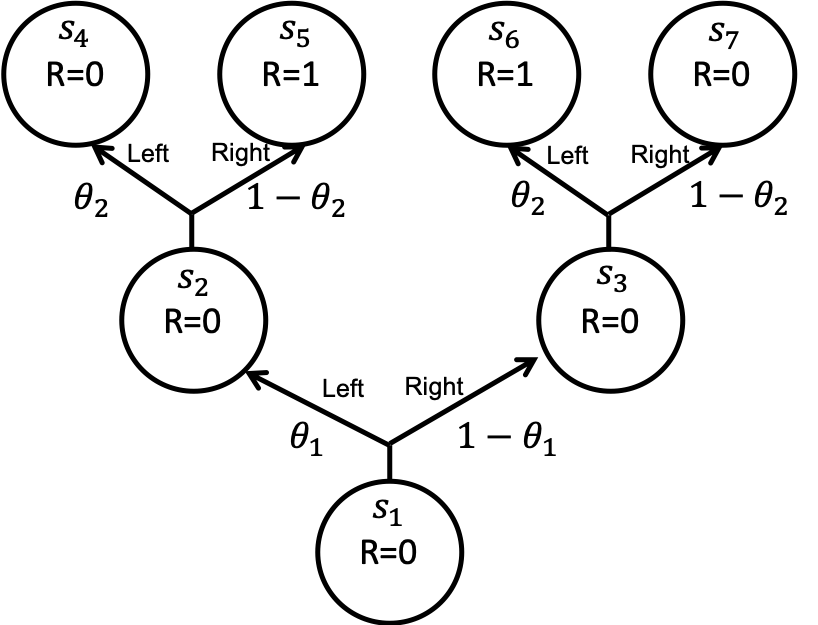
\includegraphics[width=0.5\textwidth]{figures/policy_diff.png}
    \caption{Example MDP}
    \label{fig:policy-diff-example}
\end{figure}

Intuitively, we expect that if the difference $\pi' - \pi$ is `small', then the difference in the state visitation frequencies $\discdist^{\policy'} - \discdist^{\policy}$ would also be `small', allowing us to safely replace $\discdist^{\policy'}$ in the right hand side of Eq.~\ref{eq:policy_perf_diff} with $\discdist^{\policy}$. This is the route taken by several algorithmic approaches, which differ in the way of defining a `small' policy perturbation. Of particular interest to us is the case of an infinitesimal perturbation, that is, the \textit{policy gradient} $\nabla_{\theta} J(\theta)$. In the following, we shall describe in detail several algorithms for estimating the policy gradient.

% \begin{theorem}\label{thm:policy_gradient_direct}
%     We have that
%     \begin{equation*}
%         \nabla J(\theta) = \sum_{\state} \discdist^{\policy}(\state) \sum_\action \nabla \policy(\action|\state)\QValue^{\policy}(\state,\action).
%     \end{equation*}
% \end{theorem}
% \begin{proof}
%     For simplicity we consider that θ\theta is a scalar; the extension to the vector case is immediate.
%     By definition we have that
%     \begin{equation*}
%         \begin{split}
%             \frac{\partial J(\theta)}{\partial \theta} &= \lim_{\delta \theta \to 0} \frac{J(\theta+ \delta \theta) - J(\theta)}{\delta \theta} \\
%             &=\lim_{\delta \theta \to 0} \frac{\sum_{\state} \discdist^{\policy_{\theta+ \delta \theta}}(\state) \sum_\action \policy_{\theta+ \delta \theta}(\action|\state)\left( \QValue^{\policy_{\theta}}(\state,\action) - \Value^{\policy_{\theta}}(\state)\right)}{\delta \theta}\\
%             &= \lim_{\delta \theta \to 0} \frac{\sum_{\state} \discdist^{\policy_{\theta+ \delta \theta}}(\state) \sum_\action \left(\policy_{\theta+ \delta \theta}(\action|\state) - \policy_{\theta}(\action|\state)\right) \QValue^{\policy_{\theta}}(\state,\action)}{\delta \theta}\\
%             &= \sum_{\state} \discdist^{\policy}(\state) \sum_\action \frac{\partial \policy(\action|\state)}{\partial \theta} \QValue^{\policy}(\state,\action),
%         \end{split}
%     \end{equation*}
% where the second equality uses Lemma ???????????????????????????????????????????????????????????????????????????\ref{lemma:perf_diff} and the third equality is since \Value\policyθ(\state)=∑\action\policyθ(\action|\state)\QValue\policyθ(\state,\action)\Value^{\policy_{\theta}}(\state) = \sum_{\action} \policy_{\theta}(\action|\state) \QValue^{\policy_{\theta}}(\state,\action).
% \end{proof}


\section{Gradient-Based Policy Optimization}
We would like to use the policy gradient to optimize the expected
return  $J(\theta)$ of the policy $\policy(\cdot|\cdot,\theta)$. We
will compute the gradient of $J(\theta)$, i.e., $\nabla_\theta
J(\theta)$. The update of the policy parameter $\theta$ is by gradient ascent,
\[
\theta_{\ttime+1}=\theta_\ttime + \alpha \nabla_{\theta_\ttime}
J(\theta_\ttime),
\]
where $\alpha$ is a learning rate. For a small enough learning rate, each update is guaranteed to increase $J(\theta)$.

In the following, we shall explore several different approaches for calculating the gradient $\nabla_{\theta} J(\theta)$ using rollouts from the MDP.

% One challenge we will have to address is to relate the global gradient, $\nabla_\theta J(\theta)$, to the local gradients, $\nabla \policy(\action|\state,\theta)$.



\subsection{Finite Differences Methods}

These methods can be used even when we do not have a representation
of the gradient of the policy or even the policy itself. This may
arise many times when we have, for example, access to an
off-the-shelf robot for which the software is encoded already in the
robot. In such cases we can estimate the gradient by introducing
perturbations in the parameters.

The simplest case is component-wise gradient estimates, which is also named \emph{coordinate ascent} . Let $e_i$ be
a unit vector, i.e., has in the $i$-th entry a value $1$ and a value
$0$ in all the other entries. The perturbation that we will add is
$\delta e_i$ for some $\delta >0$. We will use the following
approximation:
\[
\frac{\partial}{\partial \theta_i}J(\theta)\approx
\frac{\hat{J}(\theta+\delta e_i)-\hat{J}(\theta)}{\delta},
\]
where $\hat{J}(\theta)$ is unbiased estimator of $J(\theta)$. A more
symmetric approximation is sometimes better,
\[
\frac{\partial}{\partial \theta_i}J(\theta)\approx
\frac{\hat{J}(\theta+\delta e_i)-\hat{J}(\theta-\delta e_i
)}{2\delta}.
\]

The problem is that we need to average many samples of
$\hat{J}(\theta\pm\delta e_i)$ to overcome the noise. Another
weakness is that we need to do the computation per dimension. In
addition, the selection of $\delta$ is also critical. A small
$\delta$ might have a large noise rate that we need to overcome (by
using many samples). A large $\delta$ run the risk of facing the
non-linearity of $J$.

Rather then performing separately the computation and optimization per dimension, we can perform a more global approach and use a least squares estimation of the gradient.
Consider a random vector $u_i$, then we have
\[
J(\theta+\delta u_i)\approx J(\theta)+\delta u_i^\top \nabla
J(\theta) \;.
\]
We can define the following least square problem,
\[
G= \arg\min_x \sum_i (J(\theta+\delta u_i)- J(\theta)-\delta
u_i^\top x)^2,
\]
where $G$ is our estimate for $\nabla J(\theta)$.

We can reformulate the problem in matrix notation and define $\Delta
J^{(i)}=J(\theta+\delta u_i)- J(\theta)$ and $\Delta J= [\cdots ,
\Delta J^{(i)}, \cdots]^\top$. We define $\Delta \theta^{(i)}=\delta
u_i$, and the matrix $[\Delta\Theta]=[\cdots
\Delta\theta^{(i)},\cdots]^\top$, where the $i$-th row is
$\Delta\theta^{(i)}$.

We would like to solve for the gradient, i.e.,
\[
\Delta J\approx [\Delta \Theta]x\;.
\]
This is a standard least square problem and the solution is
\[
G=([\Delta \Theta]^\top [\Delta \Theta])^{-1} [\Delta\Theta]^\top
\Delta J\;.
\]

One issue that we neglected is that we actually do not a have the
value of $J(\theta)$. The solution is to solve also for the value of
$J(\theta)$.
%
We can define a matrix $M=[1, [\Delta\Theta]]$, i.e., adding a column of ones, a vector of unknowns $x=[J(\theta), \nabla J(\theta)]$, and have the target be $z=[\cdots, J(\theta+\delta u_i),\cdots]$. We can now solve for $z\approx Mx$, and this will recover an estimate also for $J(\theta)$.


\section{Policy Gradient Theorem}

The policy gradient theorem will relate the gradient of the expected
return $\nabla J(\theta)$ and the gradients of the policy $\nabla
\policy(\action|\state,\theta)$. We make the following assumption.
\begin{assumption}\label{ass:differentiable_policy}
The gradient $\nabla
\policy(\action|\state,\theta)$ exists and is finite for every $\theta \in \mathbb{R}^d$, $\state \in \States$, and $\action \in \Actions$.
\end{assumption}

We will mainly try to make sure
that we are able to use it to get estimates, and the quantities
would be indeed observable by the learner.

\begin{theorem}\label{thm:policy_gradient_direct}
    Let Assumption \ref{ass:differentiable_policy} hold. We have that
    \begin{equation*}
        \nabla J(\theta) = \sum_{\state} \discdist^{\policy}(\state) \sum_\action \nabla \policy(\action|\state)\QValue^{\policy}(\state,\action).
    \end{equation*}
\end{theorem}
\begin{proof}
    For simplicity we consider that $\theta$ is a scalar; the extension to the vector case is immediate.
    By definition we have that
    \begin{equation*}
        \begin{split}
            \frac{\partial J(\theta)}{\partial \theta} &= \lim_{\delta \theta \to 0} \frac{J(\theta+ \delta \theta) - J(\theta)}{\delta \theta} \\
            &=\lim_{\delta \theta \to 0} \frac{\sum_{\state} \discdist^{\policy_{\theta+ \delta \theta}}(\state) \sum_\action \policy_{\theta+ \delta \theta}(\action|\state)\left( \QValue^{\policy_{\theta}}(\state,\action) - \Value^{\policy_{\theta}}(\state)\right)}{\delta \theta}\\
            &= \lim_{\delta \theta \to 0} \frac{\sum_{\state} \discdist^{\policy_{\theta+ \delta \theta}}(\state) \sum_\action \left(\policy_{\theta+ \delta \theta}(\action|\state) - \policy_{\theta}(\action|\state)\right) \QValue^{\policy_{\theta}}(\state,\action)}{\delta \theta}\\
            &= \sum_{\state} \discdist^{\policy}(\state) \sum_\action \frac{\partial \policy(\action|\state)}{\partial \theta} \QValue^{\policy}(\state,\action),
        \end{split}
    \end{equation*}
\sloppy where the second equality uses Lemma \ref{lemma:perf_diff} and the third equality is since $\sum_\action \policy_{\theta+ \delta \theta}(\action|\state)\Value^{\policy_{\theta}}(\state) = \Value^{\policy_{\theta}}(\state)$, and $\Value^{\policy_{\theta}}(\state) = \sum_{\action} \policy_{\theta}(\action|\state) \QValue^{\policy_{\theta}}(\state,\action)$. The fourth equality holds by definition of the derivative, and using Assumption \ref{ass:differentiable_policy}. Note that Assumption \ref{ass:differentiable_policy} guarantees that $\policy$ is continuous in $\theta$, and therefore $P^{\policy}$ is continuous in $\theta$, and by Proposition \ref{prop:visitation_freq} we must have $\lim_{\delta \theta \to 0} \discdist^{\policy_{\theta+ \delta \theta}}(\state) = \discdist^{\policy}(\state)$.
\end{proof}

The Policy Gradient Theorem gives us a way to compute the gradient.
We can sample states from the distribution $\discdist^{\policy}$ using the
policy $\policy$. We still need to resolve the sampling of the
action. We are going to observe the outcome of only one action in
state $\state$, and the theorem requires summing over all of them!
In the following we will slightly modify the theorem so that we will
be able to use only the action $\action$ selected by the policy
$\policy$, rather than summing over all actions.

Consider the following simple identity,
\begin{equation}\label{eq:log_likelihood_trick}
\nabla f(x)=f(x)\frac{\nabla f(x)}{f(x)}=f(x)\nabla \log f(x).
\end{equation}
This implies that we can restate the Policy Gradient Theorem as the
following corollary,
\begin{corollary}[Policy Gradient Corollary] 
\label{thm:policy-gradient-corr} Consider a random rollout from the policy $\state_0,\action_0,\reward_0,\dots,\state_\termtime, \action_\termtime, \reward_\termtime$, where $\state_0 \sim \initdist$, $\action_\ttime\sim \policy(\cdot|\state_\ttime,\theta)$, $\state_{\ttime+1} \sim \transitionkernel (\cdot | \state_\ttime, \action_\ttime)$, and $\termtime$ is the termination time. We have
\begin{equation*}
\begin{split}
\nabla J(\theta) &= \sum_{\state \in \States} \discdist^{\policy}(\state) \sum_{\action\in
\Actions} \policy(\action|\state) \QValue^\policy
(\state,\action) \nabla \log \policy(\action|\state) \\
&=\mathbb{E}^\policy\left[\sum_{\ttime=0}^{\tau}\QValue^\policy (\state_\ttime,\action_\ttime)\nabla \log
\policy(\action_\ttime|\state_\ttime)\right].    
\end{split}
\end{equation*}
\end{corollary}
\begin{proof}
    The first equality is by the identity above, and the second is by definition of $\discdist^{\policy}(\state)$, similarly to Proposition \ref{prop:rollout_sampling}.
\end{proof}
Note that in the above corollary both the state $\state$ and action
$\action$ are sampled using the policy $\policy$. This avoids the need to sum over all actions, and leaves only the action selected by the policy.

We next provide some examples for the policy gradient theorem.

\begin{example}\label{example:mab_pg}
Consider an MDP with a single state $\state$ (which is also called
Multi-Arm Bandit, see
% , and is discussed in 
Chapter \ref{chapter:MAB}).
Assume we have only two actions, action $\action_1$ has expected
reward $\reward_1$ and action $\action_2$ has expected reward
$\reward_2$.

The policy $\policy$ is define with a parameter
$\theta=(\theta_1,\theta_2)$, where $\theta_i\in \reals$. Given
$\theta$ the probability of action $\action_i$ is
$p_i=e^{\theta_i}/(e^{\theta_1}+e^{\theta_2})$. We will also select
a horizon of length one, i.e., $\tHorizon=1$. This implies that
$\QValue^\policy(\state,\action_i)=\reward_i$.

In this simple case we can compute directly $J(\theta)$ and $\nabla
J(\theta)$. The expected return is simply,
\[
J(\theta)=p_1 \reward_1 + p_2 \reward_2 =
\frac{e^{\theta_1}}{e^{\theta_1}+e^{\theta_2}} \reward_1 +
\frac{e^{\theta_2}}{e^{\theta_1}+e^{\theta_2}} \reward_2
\]
Note that $\frac{\partial}{\partial \theta_1} p_1=
p_1-p_1^2=p_1(1-p_1) $ and $\frac{\partial }{\partial \theta_2} p_1=
- p_1 p_2= -p_1(1-p_1)$. The gradient is
\[
\nabla J(\theta)= \reward_1 \begin{pmatrix} p_1(1-p_1)\\
-p_1(1-p_1)\end{pmatrix} + \reward_2 \begin{pmatrix} -p_1(1-p_1)\\
p_1(1-p_1)\end{pmatrix} = (\reward_1-\reward_2) p_1(1-p_1) \begin{pmatrix}+1\\
-1\end{pmatrix}.
\]
Updating in the direction of the gradient, in the case that
$\reward_1>\reward_2$, would increase $\theta_1$ and decrease
$\theta_2$, and eventually $p_1$ will converge to $1$.

To apply the Policy gradient theorem we need to compute the
gradient,
\[
\nabla_\theta \policy(\action_1|\state;\theta) = \nabla \begin{pmatrix} p_1\\
1-p_1\end{pmatrix}=  \begin{pmatrix} p_1(1-p_1)\\
-p_1(1-p_1)\end{pmatrix}
\]
and the policy gradient theorem gives us the same expression,
\[
\nabla J(\theta) = \reward_1 \nabla
\policy(\action_1;\theta)+\reward_2 \nabla
\policy(\action_2;\theta)=\reward_1 \begin{pmatrix} p_1(1-p_1)\\
-p_1(1-p_1)\end{pmatrix} + \reward_2 \begin{pmatrix} -p_1(1-p_1)\\
p_1(1-p_1)\end{pmatrix},
\]
where we used the fact that there is only a single state $\state$,
and that $\QValue^\policy(\state,\action_i)=\reward_i$.
\end{example}

\begin{example}
Consider the following deterministic MDP. We have states
$\States=\{\state_0,\state_1,\state_2,\state_3\}$ and actions
$\Actions=\{\action_0,\action_1\}$. We start at $\state_0$. Action
$\action_0$ from any state leads to $\state_3$. Action $\action_1$
moves from $\state_0$ to $\state_1$, from $\state_1$ to $\state_2$ and from $\state_2$ to $\state_3$. All the rewards are zero except the terminal reward at
$\state_2$ which is $1$. The horizon is $\tHorizon=2$. This implies
that the optimal policy performs in each state $\action_1$ and has a
return of $1$.

We have a log-linear policy parameterized by $\theta\in\reals^4$. In
state $\state_0$ it selects action $\action_1$ with probability
$p_1=e^{\theta_1}/(e^{\theta_1}+e^{\theta_2})$, and in state
$\state_1$ it selects action $\action_1$ with probability
$p_2=e^{\theta_3}/(e^{\theta_3}+e^{\theta_4})$.

For this simple MDP we can specify the expected return
$J(\theta)=p_1p_2$. We can also compute the gradient and have
\[
\nabla J(\theta)=\begin{pmatrix}p_1(1-p_1)p_2\\
-p_1(1-p_1)p_2 \\  p_1 p_2 (1-p_2) \\ -p_1 p_2 (1-p_2)\end{pmatrix}= p_1 p_2\begin{pmatrix}(1-p_1)\\
-(1-p_1) \\  (1-p_2) \\ - (1-p_2)\end{pmatrix}.
\]
The policy gradient theorem will use the following ingredients. The
$\QValue^\policy$ is: $\QValue^\policy(\state_0,\action_1)=p_2$,
$\QValue^\policy(\state_1,\action_1)=1$ and all the other entries are
zero. The weights of the states are $\discdist^{\policy}(\state_0)=1$,
$\discdist^{\policy}(\state_1)=p_1$, $\discdist^{\policy}(\state_2)=p_1 p_2$ and
$\discdist^{\policy}(\state_3)=2-p_1-p_1 p_2$. The gradient of the action in each
state is:
\[
\nabla \policy(\action_1|\state_0;\theta)=
p_1\begin{pmatrix}1\\0\\0\\0\end{pmatrix} - p^2_1
\begin{pmatrix}1\\0\\0\\0\end{pmatrix} - p_1(1-p_1)
\begin{pmatrix}0\\1\\0\\0\end{pmatrix} = p_1(1-p_1)\begin{pmatrix}1\\-1\\0\\0\end{pmatrix}.
\]
Similarly
\[
\nabla \policy(\action_1|\state_1;\theta)=
p_2\begin{pmatrix}0\\0\\1\\0\end{pmatrix} - p_2^2
\begin{pmatrix}0\\0\\1\\0\end{pmatrix} - p_2(1-p_2)
\begin{pmatrix}0\\0\\0\\1\end{pmatrix} = p_2(1-p_2)\begin{pmatrix}0\\0\\1\\-1\end{pmatrix}.
\]
The policy gradient theorem states that the expected return gradient
is
\[
\discdist^{\policy}(\state_0)\QValue^\policy(\state_0,\action_1)\policy(\action_1|\state_0;\theta)
\nabla \log \policy(\action_1|\state_0;\theta) +
\discdist^{\policy}(\state_1)\QValue^\policy(\state_1,\action_1)\policy(\action_1|\state_1;\theta)
\nabla \log \policy(\action_1|\state_1;\theta),
\]
where we dropped all the terms that evaluate to zero. Plugging in
our values we have
\[
p_2 p_1 (1-p_1)\begin{pmatrix}1\\-1\\0\\0\end{pmatrix} + p_1 p_2
(1-p_2)\begin{pmatrix}0\\0\\1\\-1\end{pmatrix} = p_1 p_2\begin{pmatrix}(1-p_1)\\
-(1-p_1) \\  (1-p_2) \\ - (1-p_2)\end{pmatrix},
\]
which is identical to $\nabla J(\theta)$.
\end{example}

\begin{example}\label{example:gaussian_bandit}
    Consider the bandit setting with continuous action $\Actions = \mathbb{R}$, where the MDP has only a single state and the horizon is $\tHorizon=1$. The policy and reward are given as follows:
\begin{equation*}
    \begin{split}
        \reward(\action) &= \action, \\
        \policy(\action) &= \frac{1}{\sqrt{2 \pi \sigma^2}} \exp \left(- \frac{(\action - \theta)^2}{2 \sigma^2}\right),
    \end{split}
\end{equation*}
where the parameter is $\theta\in\reals$ and $\sigma$ is fixed and known.
As in Example \ref{example:mab_pg}, we have that $\QValue^\policy(\state,\action)=\action$. 
Also, $J(\theta) = \mathbb{E}^{\policy}[\action] = \theta$, and thus $\nabla J(\theta) = 1.$
Using Corollary \ref{thm:policy-gradient-corr}, we calculate:
\begin{equation*}
    \begin{split}
        \nabla \log \policy(\action) &= \frac{\action - \theta}{\sigma^2}, \\
        \nabla J(\theta) &= \mathbb{E}^{\policy} \left[\frac{\action(\action - \theta)}{\sigma^2}\right] 
        = \frac{1}{\sigma^2} \left(\mathbb{E}^{\policy} [\action^2] - (\mathbb{E}^{\policy} [\action])^2\right) = 1.
    \end{split}
\end{equation*}
Note the intuitive interpretation of the policy gradient here: we average the difference of an action from the mean action $\action-\theta$ and the value it yields $\QValue^\policy(\state,\action)=\action$. In this case, actions above the mean lead to higher reward, thereby `pushing' the mean action $\theta$ to increase. Note that indeed the optimal value of $\theta$ is infinite.
\end{example}

\section{Policy Gradient Algorithms}

The policy gradient theorem, and Corollary \ref{thm:policy-gradient-corr} provide a straightforward approach to estimating the policy gradient from sample rollouts: all we need to know is how to calculate $\nabla\log
\policy(\action|\state)$, and $\QValue^\policy
(\state,\action)$. In the following, we show how to compute $\nabla\log
\policy(\action|\state)$ for several policy classes. Later, we shall discuss how to estimate $\QValue^\policy
(\state,\action)$ and derive practical algorithms.

\paragraph{Log-linear policy}
For the log-linear policy class,  we have 
% $\log
% \policy(\action|\state)\propto \phi(\state,\action)^\top \theta$,
\[
\nabla \log \policy(\action|\state;\theta)= \phi(\state,\action) - \sum_{\action'}\policy(\action'|\state;\theta)\phi(\state,\action').
%-\sum_b \policy(b|\state;\theta) \phi(\state,b)
\]
% and the update is $\Delta\theta \propto \alpha U
% \phi(\state,\action)$ where $E[U]=Q^\policy(\state,\action)$.
%and$v=\sum_b \policy(b|\state;\theta) \phi(\state,b)$.
%\footnote{We have $\log \policy(\action|\state;\theta) =  $}

\paragraph{Gaussian policy} For the Gaussian policy class, we have \[
\nabla \log
\policy(\action|\state;\theta) = 
\left(\frac{\action-\xi(\state)}{\sigma^2}\right) \nabla \xi(\state).
\]
% and update is
% $\Delta\theta \propto \alpha U
% (\action-\xi(\state))\phi(\state)/\sigma^2$ where
% $E[U]=Q^\policy(\state,\action)$.

\paragraph{Simplex policy} For the Simplex policy class, we have 
\[
\nabla_{\theta_{\state,\action}} \log
\policy(\action|\state;\theta) = \nabla \log \theta_{\state,\action} - \nabla\log \sum_b \theta_{\state,b}=
\frac{1}{\theta_{\state,\action}}-\frac{1}{\sum_b \theta_{\state,b}},
\]
and for $b'\neq \action$,
\[
\nabla_{\theta_{\state,b'}} \log
\policy(\action|\state;\theta) =  - \nabla\log \sum_b \theta_{\state,b}=
-\frac{1}{\sum_b \theta_{\state,b}}.
\]

% The main benefit of the policy gradient theorem is that we do not
% need to compute either $\xi(\state)$ or $Q^\policy$. We simply run
% policy $\policy$ which visits each state $\state$ an expected
%  $\xi(\state)$ times, and let $\policy$ select
% actions. We substitute for $Q^\policy$ and unbiased random variable
% with the same value. The only thing that we need to explicitly
% compute is the gradient $\nabla \policy(\action|\state;\theta)$
% which depends on our parametrization. In the next section we couple
% the policy gradient theorem with Monte-Carlo updates to derive the
% REINFORCE algorithm.


\subsection{REINFORCE: Monte-Carlo updates}

The REINFORCE algorithm uses Monte-Carlo updates to estimate $\QValue^\policy
(\state,\action)$ in the policy gradient computation. Given a rollout
$(\state_0,\action_0,\reward_0,\state_1,\action_1,\reward_1, \ldots ,
\state_\tau,\action_\tau,\reward_\tau)$ from the policy, note that
\begin{equation*}
    \QValue^\policy
(\state_{\ttime},\action_{\ttime}) = \mathbb{E}^{\pi}\left[ \sum_{i=\ttime}^\tau \reward_i \right]. 
\end{equation*}
Therefore, let $R_{\ttime:\tau}=\sum_{i=\ttime}^\tau \reward_i$, and at each iteration REINFORCE samples a rollout and updates the policy in the direction 
$
\sum_{\ttime=0}^{\tau} R_{\ttime:\tau} \nabla \log
\policy(\action_\ttime|\state_\ttime;\theta).
$
\footnote{We implicitly assume that no state appears twice in the trajectory, and therefore the `every visit' and `first visit' Monte-Carlo updates are equivalent.}

\begin{algorithm}[H]
\caption{REINFORCE}\label{alg:reinforce}
\begin{algorithmic}[1]
\State \textbf{Input} step size $\alpha$
\State \textbf{Initialize} $\theta_0$ arbitrarily
\State \textbf{For} $j = 0,1,2,\dots$
\State \quad Sample rollout $(\state_0, \action_0, \reward_0, \ldots, \state_\tau, \action_\tau, \reward_\tau)$ using policy $\policy_{\theta_j}$.
\State \quad Set $R_{\ttime:\tau} = \sum_{i=\ttime}^\tau \reward_i$
\State \quad Update policy parameters:
    \[
    \theta_{j+1} = \theta_j + \alpha \sum_{\ttime=0}^{\tau} R_{\ttime:\tau} \nabla \log \policy(\action_\ttime | \state_\ttime; \theta_j)
    \]
\end{algorithmic}
\end{algorithm}

\subsection*{Baseline function}
One caveat with the REINFORCE algorithm as stated above, is that is tends to have high variance in estimating the policy gradient, which in practice leads to slow convergence. A common and elegant technique to reduce variance is to to add to REINFORCE a baseline function, also termed a `control variate'.

The baseline function $b(\state)$ can depend in an arbitrary way on
the state, but does not depend on the action. The main observation
would be that we can add or subtract any such function from our
$\QValue^\policy
(\state,\action)$ estimate, and it will still be unbiased. This follows since
\begin{equation}\label{eq:no_bias_trick}
\sum_\action b(\state) \nabla
\policy(\action|\state;\theta)=b(\state)\nabla \sum_\action
\policy(\action|\state;\theta)=b(\state)\nabla 1=0.
\end{equation}
Given this, we can restate the Policy Gradient Theorem as,
\[
\nabla J(\theta) = \sum_{\state \in \States} \discdist^{\policy}(\state) \sum_{\action\in
\Actions} \policy(\action|\state) \left(\QValue^\policy
(\state,\action) - b(\state)\right)\nabla \log \policy(\action|\state).
\]
This gives us a degree of freedom to select $b(\state)$. Note that
by setting $b(\state)=0$ we get the original theorem. However, we can select $b(\state)$ in a way that makes estimating the gradient easier, for example, by reducing the variance of the estimator.
\begin{proposition}
    The variance of $\nabla J(\theta)$ is minimized by $b(\state) = \frac{\sum_{\action\in\Actions} \policy(\action|\state) \left(\nabla \log \policy(\action|\state)\right)^2 \QValue^\policy(\state,\action)}{\sum_{\action\in\Actions} \policy(\action|\state) \left(\nabla \log \policy(\action|\state)\right)^2}$.
\end{proposition}
\begin{proof}
Consider the random variable $\left(\QValue^\policy(\state,\action) - b(\state)\right)\nabla \log \policy(\action|\state)$. Its expectation is $\nabla J(\theta)$, for any $b(\state)$. Its variance is $$
\sum_{\state \in \States} \discdist^{\policy}(\state) \sum_{\action\in\Actions} \policy(\action|\state) \left(\left(\QValue^\policy(\state,\action) - b(\state)\right)\nabla \log \policy(\action|\state)\right)^2 - \left(\nabla J(\theta)\right)^2.
$$
Taking a gradient with respect to $b(\state)$ and equating to $0$ gives:
\begin{equation*}    
\begin{split}
    0 &= \discdist^{\policy}(\state) \sum_{\action\in\Actions} \policy(\action|\state) \left(\nabla \log \policy(\action|\state)\right)^2 2 \left(b(\state) - \QValue^\policy(\state,\action)\right) \\
    b(\state) &= \frac{\sum_{\action\in\Actions} \policy(\action|\state) \left(\nabla \log \policy(\action|\state)\right)^2 \QValue^\policy(\state,\action)}{\sum_{\action\in\Actions} \policy(\action|\state) \left(\nabla \log \policy(\action|\state)\right)^2}.
\end{split}
\end{equation*}
\end{proof}
In many cases it is reasonable to use for $b(\state)$ the value of the state,
i.e., $b(\state)=\Value^\policy(\state)$. If we assume that the
magnitude of the gradients $|\nabla
\log \policy(\action|\state)|$ is similar for all actions
$\action\in \Actions$, the variance is minimized 
% we are left with $\mathbb{E}^\policy[(Q^\policy(\state,\action)-b(\state))^2]$ which is minimized 
by
$b(\state)=\mathbb{E}^\policy[Q^\policy(\state,\action)]=\Value^\policy(\state)$.
The following example shows an explicit case for this.
\begin{example}
    Consider the bandit setting of Example \ref{example:gaussian_bandit}, where we recall that
$        \reward(\action) = \action, \quad
        \policy_\theta(\action) = \frac{1}{\sqrt{2 \pi \sigma^2}} \exp (- \frac{(\action - \theta)^2}{2 \sigma^2}).$
Find a fixed baseline $b$ that minimizes the variance of the policy gradient estimate.

The policy gradient formula in this case is:
\begin{equation*}
        \nabla_\theta J(\theta) = \mathbb{E} \left[\frac{(\action-b)(\action - \theta)}{\sigma^2}\right] = 1, 
\end{equation*}
and we can calculate the variance
\begin{equation*}
\begin{split}
        \frac{1}{\sigma^4}\textrm{Var}\left[(\action-b)(\action - \theta)\right]  
        &=\frac{1}{\sigma^4}\mathbb{E}\left[\left((\action-b)(\action - \theta)\right)^2 - 1\right] \\
        &=\frac{1}{\sigma^4}\mathbb{E}\left[\left((\action-\theta)(\action - \theta) + (\theta-b)(\action - \theta)\right)^2 - 1\right] \\
        &=\frac{1}{\sigma^4}\mathbb{E}\left[(\action-\theta)^4 + 2(\theta-b)(\action - \theta)^3 + (\theta-b)^2(\action - \theta)^2 - 1\right] \\
        &=\frac{1}{\sigma^4}\mathbb{E}\left[(\action-\theta)^4 + (\theta-b)^2(\action - \theta)^2 - 1\right],
\end{split}
\end{equation*}
which is minimized for $b=\theta = \Value^{\policy}(\state)$.
\end{example}

We are left with the challenge of approximating
$\Value^\policy(\state)$. On the one hand this is part of the
learning. On the other hand we have developed tools to address this
in the previous chapter on value function approximation (Chapter~\ref{chapter:function-approximation}). We can use
$\Value^\policy(\state)\approx \widehat{\Value}(\state;\weight)=b(\state)$. The
good news is that any $b(\state)$ will keep the estimator unbiased,
so we do not depend on $\widehat{\Value}(\state;\weight)$ to be unbiased.

We can now describe the REINFORCE algorithm with baseline function.
We will use a Monte-Carlo sampling to estimate
$\Value^\policy(\state)$ using a class of value approximation functions $\widehat{\Value}(\cdot;\weight)$ and this will define our baseline function
$b(\state)$. Note that now we have two parameter vectors: $\theta$ for the policy, and $\weight$ for the value function.
% We will update using $U-b(\state)$ where
% $E[U]=Q^\policy(\state,\action)$. More specifically, our algorithm
% will have a class of value approximation function $V(\cdot;\weight)$
% and a parameterized policy $\policy(\cdot|\cdot;\theta)$, and in
% addition to step size parameters, $\alpha,\beta>0$. 
% Given a rollout
% $(\state_0,\action_0,\reward_0,
% \ldots,\state_\tau,\action_\tau,\reward_\tau)$, we update the parameters according to:
% \begin{equation*}
%     \begin{split}
%         R_{\ttime:\tau}&=\sum_{i=\ttime}^\tau \reward_i\\
%         \Gamma_\ttime &= R_{\ttime:\tHorizon}-V(\state_\ttime;\weight) \\
%         \theta &\leftarrow \theta + \alpha \sum_{\ttime=0}^{\tau} \Gamma_\ttime \nabla_{\theta} \log
% \policy(\action_\ttime|\state_\ttime;\theta)\\
% \weight &\leftarrow \weight + \beta \sum_{\ttime=0}^{\tau} \Gamma_\ttime \nabla_{\weight} V(\state_\ttime;\weight),
%     \end{split}
% \end{equation*}

\begin{algorithm}[H]
\caption{REINFORCE with Value Baseline}
\begin{algorithmic}[1]
\State \textbf{Input} step sizes $\alpha,\beta$
\State \textbf{Initialize} $\theta_0, \weight_0$ arbitrarily
\State \textbf{For} $j = 0,1,2,\dots$
\State \quad Sample rollout $(\state_0, \action_0, \reward_0, \ldots, \state_\tau, \action_\tau, \reward_\tau)$ using policy $\policy_{\theta_j}$.
\State \quad Set $R_{\ttime:\tau} = \sum_{i=\ttime}^\tau \reward_i$
\State \quad Set $\Gamma_\ttime = R_{\ttime:\tau}-\widehat{\Value}(\state_\ttime;\weight_j)$
\State \quad Update policy parameters:
\[
\theta_{j+1} = \theta_j + \alpha \sum_{\ttime=0}^{\tau} \Gamma_\ttime \nabla_\theta \log \policy(\action_\ttime | \state_\ttime; \theta_j).
\]
\State \quad Update value parameters:
\[
\weight_{j+1} = \weight_j + \beta \sum_{\ttime=0}^{\tau} \Gamma_\ttime \nabla_{\weight} \widehat{\Value}(\state_\ttime;\weight_j).
\]
\end{algorithmic}
\end{algorithm}

Note that the update for $\theta$ follows the policy gradient theorem with a baseline $\widehat{\Value}(\state_\ttime;\weight)$, and the update for $\weight$ is a stochastic gradient descent on the mean squared error with step size $\beta$.

% for each $\ttime\in [1,\tHorizon]$ we
% compute the $R_{\ttime:\tHorizon}$ during the times $[\ttime,\tHorizon]$, i.e.,
% $R_{\ttime:\tHorizon}=\sum_{i=\ttime}^\tHorizon \reward_i$. The error in time $\ttime$ is
% $\Gamma_\ttime=R_{\ttime:\tHorizon}-V(\state_\ttime;\weight)$. The updates
% are
% \[
% \Delta w=\alpha \Gamma_\ttime \nabla V(\state_\ttime;\weight)
% \]
% and
% \[
% \Delta \theta=\beta\Gamma_\ttime \nabla \log
% \policy(\action_\ttime|\state_\ttime;\theta)
% \]


\subsection{TD Updates and Compatible Value Functions}

In the REINFORCE algorithm above, the term $R_{\ttime:\tau}$ can be a very noisy estimate of $\QValue^\policy
(\state_{\ttime},\action_{\ttime})$, due to the stochasticity of the state transitions and action selections at times $\ttime:\tau$. A natural alternative that reduces this variance is to use bootstrapping, i.e., $\reward_{\ttime} + \Value^{\policy}(\state_{\ttime+1})$, which variance is only due to the stochasticity of the state transition at time $\ttime$. Of course, we cannot expect to have an accurate estimate of $\Value^{\policy}(\state_{\ttime+1})$ and must approximate it which, as we shall see, may induce a bias. In this section we investigate this approach, also known as the actor-critic algorithm.

% We can extend the policy gradient algorithm to handle also TD updates, using an
% actor-critic approach. We will use $\QValue$-value updates for this
% (but can be done similarly with $\Value$-values).

The critic maintains an approximate value function $\widehat{\Value}(\state;\weight)$. For each time $\ttime$ it defines the TD error to be $\Gamma_\ttime = \reward_\ttime +\widehat{\Value}(\state_{\ttime+1};\weight)-\widehat{\Value}(\state_\ttime;\weight)$. The critic's update of the value function parameters, following the TD(0) algorithm will be $\Delta w=\alpha\Gamma_\ttime \nabla \widehat{\Value}(\state_\ttime;\weight)$. The critic sends the TD error to the actor, which maintains a policy $\policy$ parameterized by $\theta$. Given a TD error $\Gamma_\ttime$, the actor updates the policy parameters by $\Delta \theta= \beta \Gamma_\ttime \nabla \log \policy(\action_\ttime|\state_\ttime;\theta)$. 

\begin{algorithm}[H]
\caption{ACTOR-CRITIC}\label{alg:actor_critic}
\begin{algorithmic}[1]
\State \textbf{Input} step sizes $\alpha,\beta$
\State \textbf{Initialize} $\theta_0, \weight_0$ arbitrarily
\State \textbf{For} $j = 0,1,2,\dots$
\State \quad Sample rollout $(\state_0, \action_0, \reward_0, \ldots, \state_\tau, \action_\tau, \reward_\tau)$ using policy $\policy_{\theta_j}$.
\State \quad Set $\Gamma_\ttime = \reward_\ttime + \widehat{\Value}(\state_{\ttime+1};\weight_j) -\widehat{\Value}(\state_\ttime;\weight_j)$
\State \label{line:actor_update}\quad ACTOR: Update policy parameters:
\[
\theta_{j+1} = \theta_j + \alpha \sum_{\ttime=0}^{\tau} \Gamma_\ttime \nabla_\theta \log \policy(\action_\ttime | \state_\ttime; \theta_j).
\]
\State \quad CRITIC: Update value parameters:
\[
\weight_{j+1} = \weight_j + \beta \sum_{\ttime=0}^{\tau} \Gamma_\ttime \nabla_{\weight} \widehat{\Value}(\state_\ttime;\weight_j).
\]
\end{algorithmic}
\end{algorithm}

% The critic maintains an approximate $\QValue$ function $\widehat{\QValue}(\state,\action;\weight)$. For each time $\ttime$ it defines the TD error to be $\Gamma_\ttime = \reward_\ttime +\widehat{\QValue}(\state_{\ttime+1},\action_{\ttime+1};\weight)-\widehat{\QValue}(\state_\ttime,\action_\ttime;\weight)$. The update will be $\Delta w=\alpha\Gamma_\ttime \nabla \widehat{\QValue}(\state_\ttime,\action_\ttime;\weight)$. The critic sends the actor the TD error $\Gamma_\ttime$.

% The actor maintains a policy $\policy$ which is parameterized by $\theta$. Given a TD error $\Gamma_\ttime$ it updates $\Delta \theta= \beta \Gamma_\ttime \nabla \log \policy(\action_\ttime|\state_\ttime;\theta)$. Then it selects $\action_{\ttime+1}\sim \policy(\cdot|\state_{\ttime+1};\theta)$.

% We need to be careful in the way we select the function
% approximation $\widehat{\QValue}(\cdot;\weight)$ since it 

Note that in contrast to REINFORCE that used the function approximation to estimate only a baseline, here our estimate of  $\reward_{\ttime} + \widehat{\Value}(\state_{\ttime+1};\weight)$ is used to estimate $\QValue^\policy
(\state_{\ttime},\action_{\ttime})$ directly, and therefore might introduce a bias due to an inaccurate approximation.
% (note that here we use the function approximation to estimate $\QValue(\state,\action)$ directly, and not the baseline as in the REINFORCE method above).


Interestingly, there is a special case for which it is guaranteed
that we will not have such a bias. The following theorem established this result; for simplicity we use an approximation of $\widehat{\QValue}(\state_{\ttime}, \action_{\ttime};\weight)$ instead of $\reward_{\ttime} + \widehat{\Value}(\state_{\ttime+1};\weight)$.

Let the expected square error of $\weight$ be
\[
SE(\weight)=\frac{1}{2}\mathbb{E}^\policy[(\QValue^\policy(\state,\action)-\widehat{\QValue}(\state,\action;\weight))^2].
\]
A value function is {\em compatible} if,
\[
\nabla_\weight \widehat{\QValue}(\state,\action;\weight)= \nabla_\theta
\log \policy(\action|\state;\theta).
\]


\begin{theorem}
Assume that $\widehat{\QValue}$ is compatible and $\weight$ minimizes $SE(\weight)$,
then,
\[
\nabla_\theta J(\theta)=\sum_{\ttime=1}^\tau \mathbb{E}^\policy[\widehat{\QValue}(\state_\ttime,\action_\ttime;\weight)
\nabla \log \policy(\action_\ttime|\state_\ttime;\theta)].
\]
\end{theorem}

\begin{proof}
Since $\weight$ minimizes $SE(\weight)$ we have
\begin{align*}
0 & = \nabla_\weight SE(\weight)\\
&= \nabla_\weight \mathbb{E}^\policy[(\QValue^\policy(\state,\action)-\widehat{\QValue}(\state,\action;\weight))^2]\\
&=
\mathbb{E}^\policy[(\QValue^\policy(\state,\action)-\widehat{\QValue}(\state,\action;\weight))\nabla_\weight
\widehat{\QValue}(\state,\action;\weight)].
\end{align*}
Since $\widehat{\QValue}$ is compatible, we have $\nabla_\weight
\widehat{\QValue}(\state,\action;\weight)= \nabla_\theta \log
\policy(\action|\state;\theta)$ which implies,
\begin{align*}
0&=
\mathbb{E}^\policy[(\QValue^\policy(\state,\action)-\widehat{\QValue}(\state,\action;\weight))\nabla_\theta
\log \policy(\action|\state;\theta)],
\end{align*}
and have
\begin{align*}
\mathbb{E}^\policy[\QValue^\policy(\state,\action)\nabla_\theta \log \policy(\action|\state;\theta)] = \mathbb{E}^\policy[\widehat{\QValue}(\state,\action;\weight)\nabla_\theta \log \policy(\action|\state;\theta)].
\end{align*}
This implies that by substituting $\QValue$ in the policy gradient theorem
we have
\[
\nabla_\theta J(\theta) = \sum_{\ttime=1}^\tau \mathbb{E}^\policy[\widehat{\QValue}(\state,\action;\weight)
\nabla \log \policy(\action|\state;\theta)].
\]
\end{proof}

For non-compatible function approximation, we can combine the zero-bias, high-variance REINFORCE update with the biased but low-variance ACTOR-CRITIC update using the idea of TD with multi-step lookahead (see Chapter \ref{sec:TD_lambda}). Recall that we defined multi-step TD as:
\begin{equation*}
    \begin{split}
        \Gamma^{(0)}_\ttime &= \reward_{\ttime} + \widehat{\Value}(\state_{\ttime+1};\weight) - \widehat{\Value}(\state_{\ttime};\weight), \\
        \Gamma^{(1)}_\ttime &= \reward_{\ttime} + \reward_{\ttime+1} + \widehat{\Value}(\state_{\ttime+2};\weight) - \widehat{\Value}(\state_{\ttime};\weight), \\
        & \dots \\
        \Gamma^{(n)}_\ttime &= \reward_{\ttime} + \reward_{\ttime+1} + \dots + \reward_{\ttime+n-1} + \widehat{\Value}(\state_{\ttime+n};\weight) - \widehat{\Value}(\state_{\ttime};\weight),
    \end{split}
\end{equation*}
and the TD($\lambda$) update in this case can defined as 
$\Gamma^{\lambda}_\ttime = \frac{1}{Z_\ttime}\sum_{n=1}^{\tau - \ttime}
\lambda^{n-1}\Gamma^{(n)}_\ttime,$ where the normalizing constant $Z_\ttime = \sum_{n=1}^{\tau - \ttime}
\lambda^{n-1}$.  

Note that for $\lambda = 0$ we obtain the standard ACTOR-CRITIC update above, while for $\lambda = 1$ the update puts almost all of the weight on $\Gamma^{(n)}_\ttime$, which is equivalent to REINFORCE (since we consider an episodic MDP and not a discounted setting, the horizon is not infinite and therefore the equivalence of TD($1$) to REINFORCE is only an approximation). By choosing $\lambda$ between $0$ and $1$ we can balance between bias and variance. Using $\Gamma^{\lambda}_\ttime$ instead of $\Gamma_\ttime$ in the actor update (line \ref{line:actor_update} in Algorithm \ref{alg:actor_critic}) is also known as \textit{generalized advantage estimation}.




% We can summarize the various updates for the policy gradient as
% follows:
% \begin{itemize}
% \item REINFORCE (which is a Monte-Carlo estimate) uses
% $\mathbb{E}^\policy[R_\ttime \nabla\log\policy(\action|\state;\theta) ]$.
% \item $\QValue$-function with actor-critic uses
% $\mathbb{E}^\policy[\widehat{\QValue}(\action_\ttime|\state_\ttime;\weight)
% \nabla\log\policy(\action|\state;\theta) ]$.
% \item A-function with actor-critic uses
% $\mathbb{E}^\policy[A(\action_\ttime|\state_\ttime;\weight)
% \nabla\log\policy(\action|\state;\theta) ]$, where
% $A(\action|\state;\weight)=\widehat{\QValue}(\state,\action;\weight)-\widehat{\Value}(\state;\weight)$. The A-function is also called the \emph{Advantage function}.
% \item TD with actor-critic uses
% $\mathbb{E}^\policy[\Gamma\nabla\log\policy(\action|\state;\theta) ]$, where
% $\Gamma$ is the TD error.
% \end{itemize}

\section{Convergence of Policy Gradient}

As our policy optimization in this chapter is based on gradient descent, it is important to understand whether it converges, and what it converges to. As illustrated in Figure \ref{fig:gradient_descent}, we can only expect gradient descent to converge to a globally optimal solution for functions that do not have sub-optimal local minima. The policy parametrization itself may induce local optima, and in this case there is no reason to expect convergence to a globally optimal policy. However, let us consider the case where the policy parameterization is expressive enough to not directly add local minima to the loss landscape, such as the simplex policy structure above. Will policy gradeint converge to a globally optimal policy in this case?

Convex functions do not have local minima. However, as the following example shows, MDPs are not necessarily convex (or concave) in the policy, regardless of the policy parameterization.

\begin{figure}[h]
    \centering
    \begin{subfigure}[b]{0.3\textwidth}
        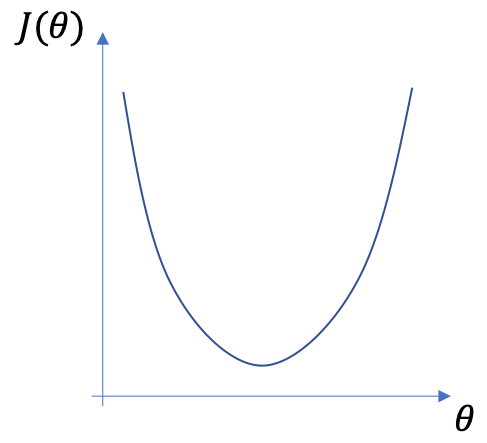
\includegraphics[width=\textwidth]{figures/convex_function.png}
        \caption{A convex function with single global minimum.}
        \label{fig:convex}
    \end{subfigure}
    \hfill % add horizontal space between figures
    \begin{subfigure}[b]{0.3\textwidth}
        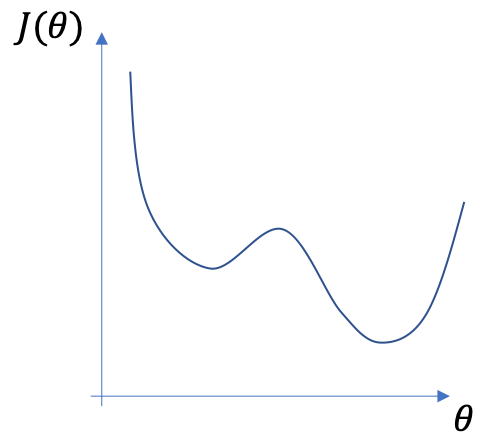
\includegraphics[width=\textwidth]{figures/non_convex_function.png}
        \caption{Non convex function with a sub-optimal local minimum.}
        \label{fig:non_convex}
    \end{subfigure}
    \hfill % add horizontal space between figures
    \begin{subfigure}[b]{0.3\textwidth}
        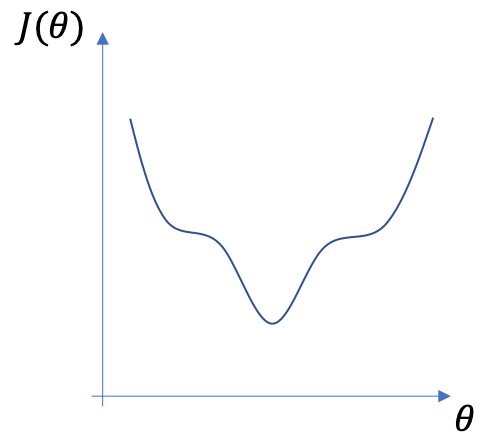
\includegraphics[width=\textwidth]{figures/converging_function.png}
        \caption{Non convex function with a single global minimum.}
        \label{fig:converging_non_convex}
    \end{subfigure}
    \caption{Gradient descent with a proper step size will converge to a global optimum in (a) and (c), but not in (b).}\label{fig:gradient_descent}
\end{figure}

\begin{example}\label{example:non_convex}
    A convex function $f(x)$ satisfies $f(\lambda x_1 + (1-\lambda) x_2) \leq \lambda f(x_1) + (1-\lambda) f(x_2)$. A concave function satisfies $f(\lambda x_1 + (1-\lambda) x_2) \geq \lambda f(x_1) + (1-\lambda) f(x_2)$.
    We will show that MDPs are not necessarily convex or concave in the policy.

    Consider an MDP with two states $\state_1, \state_2$. In $\state_1$, taking action $\action_1$ transitions to $\state_2$ with 0 reward, while action $\action_2$ terminates with 0 reward. In state $\state_2$, taking action $\action_1$ terminates with reward $0$, and taking action $\action_2$ terminates with reward $10$. Consider two policies: $\policy_1$ chooses $\action_1$ in both states, and $\policy_2$ chooses $\action_2$ in both states. We have that $\Value^{\policy_1}(\state_1) = 0$ and $\Value^{\policy_2}(\state_1) = 0$. 
    Now, consider the policy $\policy_\lambda(\action|\state) = \lambda \policy_1(\action|\state) + (1-\lambda)\policy_2(\action|\state)$. For $\lambda=0.5$ we have that $\Value^{\policy_\lambda}(\state_1) = 2.5 > \lambda \Value^{\policy_1}(\state_1) + (1-\lambda) \Value^{\policy_2}(\state_1)$, and therefore the MDP is not convex. 
    By changing the rewards in the example to be their negatives, we can similarly show that the MDP is not concave.
\end{example}

\begin{remark}
    Note that the way we combined policies in Example \ref{example:non_convex} is by combining the action probabilities \textit{at every state}. This is required for establishing convexity of the value in the policy. Perhaps a more intuitive way of combining two policies is by selecting which policy to run at the beginning of an episode, and using only that policy throughout the episode. For such a non-Markovian policy, the expected value will simply be the average of the values of the two policies.
\end{remark}

\begin{remark}
    From the linear programming formulation in Chapter \ref{chapter-discount:section:LP}, we know that the value is linear (and thereby convex) in the state-action frequencies. While a policy can be inferred from state-action frequencies, this mapping is non-linear, and as the example above shows, renders the mapping from policy to value not necessarily convex.
\end{remark}

% \YM{
% We should make a few remarks about combining policies. First, one can combine policies by either selecting initially which policy to run, and using only it. This will guarantee that the expected reward will equal the expected value functions. Note the difference between selecting only once initially, and selecting at each state, as in Example ????????????????????????\ref{example:non_convex}. Second, if we consider the state-action frequencies, the expected value is linear in this parameter, and so a convex combination of them would average the value functions. The resulting policy can be inferred from the state-action frequencies. 
% }\AT{I added two remarks. Not sure if the first one is relevant here, feel free to edit/delete them}

Following Example \ref{example:non_convex}, we should not immediately expect policy gradient algorithms to converge to a globally optimal policy. Interestingly, in the following we shall show that nevertheless, for the simplex policy there are no local optima that are not globally optimal.

Before we show this, however, we must handle a delicate technical issue. The simplex policy is only defined for $\theta_{\state,\action}\geq 0$. What happens if some $\theta_{\state,\action} = 0$ and $\frac{\partial J(\theta)}{\partial \theta_{\state,\action}} < 0$? We shall assume that in this case, the policy gradient algorithm will maintain $\theta_{\state,\action} = 0$. We can therefore consider a modified gradient at $\theta_{\state,\action} = 0$:
\begin{equation*}
    \left.\tilde{\frac{\partial J(\theta)}{\partial \theta_{\state,\action}}}\right|_{\theta_{\state,\action} = 0} = \max \left\{0, \frac{\partial J(\theta)}{\partial \theta_{\state,\action}}\right\}, \qquad \left.\tilde{\frac{\partial J(\theta)}{\partial \theta_{\state,\action}}}\right|_{\theta_{\state,\action} \neq 0} = \frac{\partial J(\theta)}{\partial \theta_{\state,\action}}.
\end{equation*}

We shall make a further assumption that $\discdist^{\policy}(\state) > 0$ for all $\state, \policy$. To understand why this is necessary, consider an initial policy $\pi_0$ that does not visit a particular state $\state$ at all, and therefore $\discdist^{\policy_0}(\state) = 0$. From the policy gradient theorem, we will have that $\frac{\partial J(\theta)}{\partial \theta_{\state,\action}} = 0$, and therefore the policy at $\state$ will not improve. If the optimal policy in other states does not induce a transition to $\state$, we cannot expect convergence to optimal policy in $\state$. In other words, the policy must \textit{explore} enough to cover the state space.

Furthermore, for simplicity, we shall assume that the optimal policy is unique.

Let us now calculate the policy gradient for the simplex policy.

\begin{equation*}
    \frac{\partial \policy(\action'|\state)}{\partial \theta_{\state,\action}} = \begin{cases}
        \frac{\sum_{\action''} \theta_{\state,\action''} - \theta_{\state,\action'}}{(\sum_{\action''} \theta_{\state,\action''})^2} & \text{if } \action' = \action, \\
\frac{ - \theta_{\state,\action'}}{(\sum_{\action''} \theta_{\state,\action''})^2} & \text{if } \action' \neq \action.
    \end{cases}
\end{equation*}

Using the policy gradient theorem,
\begin{equation*}
\begin{split}
    \frac{\partial J(\theta)}{\partial \theta_{\state,\action}}  &= \discdist^{\policy}(\state) \sum_{\action'} \frac{\partial \policy(\action'|\state)}{\partial \theta_{\state,\action}}\QValue^{\policy}(\state,\action')\\
    &= \frac{\discdist^{\policy}(\state)}{(\sum_{\action''} \theta_{\state,\action''})^2} \sum_{\action'} \left(\QValue^{\policy}(\state,\action) - \QValue^{\policy}(\state,\action') \right)\theta_{\state,\action'} \\
    &= \frac{\discdist^{\policy}(\state)}{\sum_{\action''} \theta_{\state,\action''}} \sum_{\action'} \left(\QValue^{\policy}(\state,\action) - \QValue^{\policy}(\state,\action') \right)\policy(\action'|\state) \\
    &=\frac{\discdist^{\policy}(\state)}{\sum_{\action''} \theta_{\state,\action''}}\left(\QValue^{\policy}(\state,\action) - \Value^{\policy}(\state) \right).
\end{split}  
\end{equation*}

Now, assume that $\policy$ is not optimal, therefore there exists some $\state$ for which $\max_{\action} \QValue^{\policy}(\state,\action) > \Value^{\policy}(\state)$ (otherwise, $\Value^{\policy}$ would satisfy the Bellman optimality equation and would therefore be optimal). In this case, we have that $\frac{\partial J(\theta)}{\partial \theta_{\state,\action}} > 0$ and therefore $\theta$ is not a local optimum.

Lastly, we should verify that the optimal policy $\policy^*$ is indeed a global optimum. The unique optimal policy is deterministic, and satisfies 
$$\policy^*(\action|\state) = \begin{cases}
        1 & \text{if } \QValue^{\policy^*}(\state,\action) = \Value^{\policy^*}(\state), \\
0 & \text{else }.
\end{cases}$$
Consider any $\theta^*$ such that for all $\state,\action$ satisfies $$\theta^*_{\state,\action} = \begin{cases}
        >0 & \text{if } \QValue^{\policy^*}(\state,\action) = \Value^{\policy^*}(\state), \\
0 & \text{else }.
\end{cases}$$ 
By the above, we have that for the optimal action $\frac{\partial J(\theta)}{\partial \theta_{\state,\action}} = 0$, and for non-optimal actions $\QValue^{\policy^*}(\state,\action) - \Value^{\policy^*}(\state) < 0$, therefore, $\frac{\partial J(\theta)}{\partial \theta_{\state,\action}} < 0$ and $\tilde{\frac{\partial J(\theta)}{\partial \theta_{\state,\action}}} = 0$.
% Therefore, if $\theta_{\state,\action} \neq 0$, we have that $\frac{\partial J(\theta)}{\partial \theta_{\state,\action}} = 0$ only if $\QValue^{\policy}(\state,\action) = \Value^{\policy}(\state)$

\section{Proximal Policy Optimization}

Recall our discussion about the policy difference lemma: if the difference $\policy' - \policy$ is `small', then the difference in the state visitation frequencies $\discdist^{\policy'} - \discdist^{\policy}$ would also be `small', allowing us to safely replace $\discdist^{\policy'}$ in the right hand side of Eq.~\ref{eq:policy_perf_diff} with $\discdist^{\policy}$. The Proximal Policy Optimization (PPO) algorithm is a popular heuristic that takes this approach, and has proved to perform very well empirically.


To simplify our notation we write the advantage function $\AdvValue^{\policy}(\state,\action) = \QValue^{\policy}(\state,\action) - \Value^{\policy}(\state)$. The idea is to maximize the policy that leads to policy improvement
\begin{equation*}
    \max_{\policy'\in \Pi}\sum_{\state} \discdist^{\policy'}(\state) \sum_\action \policy'(\action|\state)\AdvValue^{\policy}(\state,\action),
\end{equation*}
by replacing $\discdist^{\policy'}$ with the visitation frequencies of the current policy $\discdist^{\policy}$, and performing the search over a limited set of policies $\Pi$ that is similar to $\policy$. The main trick in PPO is that this constrained optimization can be done implicitly, by maximizing the following objective:
\begin{equation}\label{eq:PPO}
    \textrm{PPO}(\!\policy\!) \!=\! \max_{\!\policy'\!}\sum_{\!\state\!} \!\discdist^{\policy}(\state)\! \sum_{\!\action\!} \policy(\!\action|\state\!) \min \! \left\{\frac{\policy'(\!\action|\state\!)}{\policy(\!\action|\state\!)}\AdvValue^{\policy}(\!\state,\!\action\!),  \textrm{clip}\!\left(\frac{\policy'(\!\action|\state\!)}{\policy(\!\action|\state\!)}\!\!, 1 \!-\!\epsilon, 1\!+\!\epsilon\!\right)\!\!\AdvValue^{\policy}(\!\state,\!\action\!) \!\right\},
\end{equation}
where $\textrm{clip}\left(x , x_{\min}, x_{\max}\right) = \min\{\max\{x, x_{\min}\}, x_{\max}\}$,
and $\epsilon$ is some small constant. Intuitively, the clipping in this objective prevents the ratio between the new policy $\policy'(\action|\state)$ and the previous policy $\policy(\action|\state)$ to grow larger than $\epsilon$, assuring that maximizing the objective indeed leads to an improved policy.

To understand exactly how this works, consider the following two cases:
\begin{enumerate}
    \item $\AdvValue^{\policy}(\state,\action) > 0$: in this case, the $\max$ over $\policy'$ would drive to maximize $\policy'(\action|\state)$, but the $\min$ in the objective would limit $\policy'(\action|\state)$ to at most $\left( 1+\epsilon\right)\policy(\action|\state)$.
    \item $\AdvValue^{\policy}(\state,\action) < 0$: in this case, the $\max$ over $\policy'$ would drive to minimize $\policy'(\action|\state)$ to $0$, but the $\min$ in the objective would limit $\policy'(\action|\state)$ to be no smaller than $\left( 1-\epsilon\right)\policy(\action|\state)$.
\end{enumerate}

To optimize the PPO objective using a sample rollout, we let $\Gamma_\ttime$ denote an estimate of the advantage at state $\state_\ttime, \action_\ttime$, and take gradient descent steps on:
\begin{equation*}
    \nabla_{\theta}\sum_{\ttime=0}^\tau \min \left\{\frac{\policy'(\action_\ttime|\state_\ttime, \theta)}{\policy(\action_\ttime|\state_\ttime)}\Gamma_\ttime,  \textrm{clip}\left(\frac{\policy'(\action_\ttime|\state_\ttime, \theta)}{\policy(\action_\ttime|\state_\ttime)} , 1-\epsilon, 1+\epsilon\right)\Gamma_\ttime \right\}.
\end{equation*}

\begin{algorithm}[H]
\caption{PPO}
\begin{algorithmic}[1]
\State \textbf{Input} step sizes $\alpha,\beta$, inner loop optimization steps $K$, clip parameter $\epsilon$
\State \textbf{Initialize} $\theta, \weight$ arbitrarily
\State \textbf{For} $j = 0,1,2,\dots$
\State \quad Sample rollout $(\state_0, \action_0, \reward_0, \ldots, \state_\tau, \action_\tau, \reward_\tau)$ using policy $\policy$.
\State \quad Set $R_{\ttime:\tau} = \sum_{i=\ttime}^\tau \reward_i$
\State \quad Set $\Gamma_\ttime = R_{\ttime:\tau}-V(\state_\ttime;\weight)$
\State \quad Set $\theta_{prev} = \theta$
\State \quad \textbf{For} $k=1,\dots,K$
\State \quad \quad \quad Update policy parameters:
\[
\quad \quad \quad \theta := \theta + \alpha \nabla_{\theta}\sum_{\ttime=0}^\tau \min \left\{\frac{\policy(\action_\ttime|\state_\ttime, \theta)}{\policy(\action_\ttime|\state_\ttime, \theta_{prev})}\Gamma_\ttime,  \textrm{clip}\left(\frac{\policy(\action_\ttime|\state_\ttime, \theta)}{\policy(\action_\ttime|\state_\ttime, \theta_{prev})} , 1-\epsilon, 1+\epsilon\right)\Gamma_\ttime \right\}
\]
\State \quad Update value parameters:
\[
\weight := \weight + \beta \sum_{\ttime=0}^{\tau} \Gamma_\ttime \nabla_{\weight} V(\state_\ttime;\weight)
\]
\end{algorithmic}
\end{algorithm}

\section{Alternative Proofs for the Policy Gradient Theorem}\label{sec:alternative_proof}
In this section, for didactic purposes, we show two alternative proofs for the policy gradient theorem (Theorem \ref{thm:policy_gradient_direct}). The first proof is based on an elegant idea of unrolling of the value function, and the second is based on a trajectory-based view. The trajectory-based proof will also lead to an interesting insight about partially observed systems.

\subsection{Proof Based on Unrolling the Value Function}
The following is an alternative proof of Theorem \ref{thm:policy_gradient_direct}.
\begin{proof}
For each state $\state$ we have
\begin{align*}
\nabla \Value^\policy(\state) =& \nabla \sum_\action \policy(\action|\state) \QValue^\policy(\state,\action)\\
=&\sum_\action  \QValue^\policy(\state,\action) \nabla \policy(\action|\state) + \policy(\action|\state) \nabla \QValue^\policy(\state,\action)\\
=&\sum_\action  \QValue^\policy(\state,\action) \nabla \policy(\action|\state) + \policy(\action|\state) \sum_{\state_1} \transitionprob(\state_1|\state,\action) \nabla \Value^\policy(\state_1)\\
=& \sum_\action  \QValue^\policy(\state,\action) \nabla
\policy(\action|\state) + \sum_{\state_1} \transitionkernel^{\policy}(\state_1|\state)
\nabla \Value^\policy(\state_1)\\
=& \sum_\action  \QValue^\policy(\state,\action) \nabla
\policy(\action|\state) + \sum_{\state_1} \transitionkernel^{\policy}(\state_1|\state)
\sum_\action \QValue^\policy(\state_1,\action) \nabla
\policy(\action|\state_1) \\
& + \sum_{\state_1, \state_2}
\transitionkernel^{\policy}(\state_2|\state_1)\transitionkernel^{\policy}(\state_1|\state)
\nabla \Value^\policy(\state_2)\\
=& \sum_{\state\in
\States}\sum_{t=0}^\infty \Pr(\state_t = \state | \state_0 = \state, \policy) \sum_\action
\QValue^\policy(\state,\action)\nabla\policy(\action|\state),
\end{align*}
where the first identity follows since by averaging $Q^\policy(\state,\action)$ over the actions $\action$, with the
probabilities induce by $\policy(\action|\state)$, we have both correct expectation of the immediate reward and the next state is distributed correctly. The second equality follows from the gradient of a multiplication, i.e., $\nabla AB=A\nabla B+B\nabla A$. The third follows since 
$\nabla \QValue^\policy(\state,\action)= \nabla
[\reward(\state,\action)+
\sum_{\state'}\transitionkernel(\state'|\state,\action)\Value^\policy(\state'|\state,\action)]$.
%
The next two identities role the policy one step in to the future.
%
The last identity follows from unrolling $\state_1$ to $\state_2$ etc., and then reorganizing the terms. The term that depends on $\nabla \Value^\policy(\state_2)$ vanishes for $t\to\infty$ because we assume that the termination time is bounded with probability 1.

Using this we have
\begin{align*}
\nabla J(\theta) &= \nabla \sum_{\state} \initdist(\state) \Value^\policy (\state)\\
&= \sum_\state \initdist(\state) \left(\sum_{t=0}^\infty \Pr(\state_t = \state | \state_0 = \state, \policy) \right) \sum_\action \QValue^\policy (\state,\action) \nabla\policy(\action|\state) \\
&= \sum_\state \left(\sum_{t=0}^\infty \Pr(\state_t = \state | \initdist, \policy) \right) \sum_\action \QValue^\policy (\state,\action) \nabla\policy(\action|\state) \\
&= \sum_\state \discdist^{\policy}(\state) \sum_\action \nabla\policy(\action|\state) \QValue^\policy (\state,\action) ,
\end{align*}
where the last equality is by definition of $\discdist^{\policy}$.
\end{proof}


\subsection{Proof Based on the Trajectory View}

We next describe yet another proof for the policy gradient theorem, which will provide some interesting insights.

We begin by denoting by $\rollout$ a random rollout from the policy, $\rollout = \{\state_0,\action_0,\reward_0,\dots,\state_\termtime, \action_\termtime, \reward_\termtime \}$, where $\state_0 \sim \initdist$, $\action_\ttime\sim \policy(\cdot|\state_\ttime,\theta)$, $\state_{\ttime+1} \sim \transitionprob (\cdot | \state_\ttime, \action_\ttime)$, and $\termtime$ is the termination time. We also let $\reward(\rollout) = \sum_{\ttime=0}^\termtime \reward_\ttime$ denote the accumulated reward in the rollout, and $\Pr(\rollout)$ the probability of observing $\rollout$, which by our definitions is 
\begin{equation}\label{eq:rollout_prob}
\Pr(\rollout) = \initdist(\state_0)\policy(\action_0|\state_0,\theta)\transitionprob(\state_1|\state_0,\action_0)\policy(\action_1|\state_1,\theta)\cdots\transitionprob(\state_G|\state_{\termtime},\action_{\termtime}).
\end{equation}
We therefore have that
\begin{equation*}
    J(\theta) = \mathbb{E}^{\policy}\left[ \reward(\rollout) \right] = \sum_{\rollout} \Pr(\rollout) \reward(\rollout),
\end{equation*}
and, by using a similar trick to \eqref{eq:log_likelihood_trick}, we have that 
\begin{equation*}
    \nabla J(\theta) = \sum_{\rollout} \nabla \Pr(\rollout) \reward(\rollout) = \sum_{\rollout} \frac{\nabla \Pr(\rollout)}{\Pr(\rollout)} \reward(\rollout) \Pr(\rollout) = \mathbb{E}^{\policy}\left[ \nabla \log \Pr(\rollout)\reward(\rollout) \right].
\end{equation*}
We now notice that 
\begin{equation*}
\begin{split}
    \nabla \log \Pr(\rollout) &= \nabla \left( \log \initdist(\state_0) + \log \policy(\action_0|\state_0,\theta) + \log\transitionprob(\state_1|\state_0,\action_0) + \dots + \log\transitionprob(\state_G|\state_{\termtime-1},\action_{\termtime-1})\right) \\
    &= \sum_{\ttime=0}^{\termtime} \nabla\log \policy(\action_\ttime|\state_\ttime,\theta),
\end{split}
\end{equation*}
where the first equality is by \eqref{eq:rollout_prob}, and the second equality is since the transitions and initial distribution do not depend on $\theta$. We therefore have that
\begin{equation}\label{eq:pg_score_1}
    \nabla J(\theta) = \mathbb{E}^{\policy}\left[ \sum_{\ttime=0}^\termtime \nabla\log \policy(\action_\ttime|\state_\ttime,\theta) \sum_{\ttime'=0}^\termtime \reward(\state_{\ttime'},\action_{\ttime'})\right].
\end{equation}
We next show that in the sums in \eqref{eq:pg_score_1}, it suffices to only consider rewards that come after $\nabla\log \policy(\action_\ttime|\state_\ttime,\theta)$. For $\ttime' < \ttime$, we have
\begin{equation*}
\begin{split}
    \mathbb{E}^{\policy}\left[ \nabla\log \policy(\action_\ttime|\state_\ttime,\theta) \reward(\state_{\ttime'},\action_{\ttime'})\right] &= \mathbb{E}^{\policy}\left[ \mathbb{E}^{\policy}\left[\left.\nabla\log \policy(\action_\ttime|\state_\ttime,\theta) \reward(\state_{\ttime'},\action_{\ttime'})\right| \state_0,\action_0,\dots,\state_\ttime\right]\right] \\
    &= \mathbb{E}^{\policy}\left[ \reward(\state_{\ttime'},\action_{\ttime'}) \mathbb{E}^{\policy}\left[\left.\nabla\log \policy(\action_\ttime|\state_\ttime,\theta) \right| \state_0,\action_0,\dots,\state_\ttime\right]\right] = 0,
\end{split}
\end{equation*}
where the first equality is from the law of total expectation, and the last is similar to \eqref{eq:no_bias_trick}. So we have
\begin{equation}\label{eq:pg_score_2}
    \nabla J(\theta) = \mathbb{E}^{\policy}\left[ \sum_{\ttime=0}^\termtime \nabla\log \policy(\action_\ttime|\state_\ttime,\theta) \sum_{\ttime'=\ttime}^\termtime \reward(\state_{\ttime'},\action_{\ttime'})\right].
\end{equation}
Note that the REINFORCE Algorithm \ref{alg:reinforce} can be seen as estimating the expectation in \eqref{eq:pg_score_2} from a single roll out. To finally obtain the policy gradient theorem, using the law of total expectation again, we have
\begin{equation*}
\begin{split}
    \mathbb{E}^{\policy}\left[ \sum_{\ttime=0}^\termtime \nabla\log \policy(\action_\ttime|\state_\ttime,\theta) \sum_{\ttime'=\ttime}^\termtime \reward(\state_{\ttime'},\action_{\ttime'})\right] &= \mathbb{E}^{\policy}\left[ \sum_{\ttime=0}^\infty \nabla\log \policy(\action_\ttime|\state_\ttime,\theta) \sum_{\ttime'=\ttime}^\infty \reward(\state_{\ttime'},\action_{\ttime'})\right] \\
    &= \sum_{\ttime=0}^\infty \mathbb{E}^{\policy}\left[ \nabla\log \policy(\action_\ttime|\state_\ttime,\theta) \sum_{\ttime'=\ttime}^\infty \reward(\state_{\ttime'},\action_{\ttime'})\right] \\
    &=\sum_{\ttime=0}^\infty \mathbb{E}^{\policy}\left[ \mathbb{E}^{\policy}\left[ \left.\nabla\log \policy(\action_\ttime|\state_\ttime,\theta) \sum_{\ttime'=\ttime}^\infty \reward(\state_{\ttime'},\action_{\ttime'})\right| \state_\ttime, \action_\ttime\right]\right] \\
    &=\sum_{\ttime=0}^\infty \mathbb{E}^{\policy}\left[\nabla\log \policy(\action_\ttime|\state_\ttime,\theta) \mathbb{E}^{\policy}\left[ \left. \sum_{\ttime'=\ttime}^\infty \reward(\state_{\ttime'},\action_{\ttime'})\right| \state_\ttime, \action_\ttime\right]\right] \\
    &=\sum_{\ttime=0}^\infty \mathbb{E}^{\policy}\left[\nabla\log \policy(\action_\ttime|\state_\ttime,\theta) \QValue^{\policy}(\state_\ttime, \action_\ttime)\right]\\
    &=\mathbb{E}^{\policy}\left[\sum_{\ttime=0}^\termtime\nabla\log \policy(\action_\ttime|\state_\ttime,\theta) \QValue^{\policy}(\state_\ttime, \action_\ttime)\right],
\end{split}
\end{equation*}
which is equivalent to the expression in Corollary \ref{thm:policy-gradient-corr}. The first equality is since the terminal state is absorbing, and has reward zero. The justification for exchanging the expectation and infinite sum in the second equality is not straightforward. In this case it holds by the Fubini theorem, using Assumption \ref{ass:finite_termination_prob}.

\paragraph{Partially Observed States} We note that the derivation of \eqref{eq:pg_score_1} follows through if we consider policies that cannot access the state, but only some encoding $\phi$ of it, $\policy(\action|\phi(\state))$. Even though the optimal Markov policy in an MDP is deterministic, the encoding may lead to a system that is not Markovian anymore, by
coalescing certain states which have identical encoding. Considering stochastic policies and using a policy gradient approach can be beneficial in such situations, as demonstrated in the following example. 
\begin{example}[Aliased Grid-world from David Silver's course \cite{DavidSilver-course}]
    Consider the example in Figure~\ref{fig:L9-grid-world}. The green
state is the good goal and the red ones are the bad. The encoding of
each state is the location of the walls. In each state we need to
choose a direction. The problem is that we have two states which are
indistinguishable (marked by question mark).

It is not hard to see that any deterministic policy would fail from
some start state (either the left or the right one). Alternatively,
we can use a randomized policy in those states,with probability half
go right and probability half go left. For such a policy we have a
rather short time to reach the green goal state (and avoid the red
states).

The issue here was that two different states had the same encoding,
and thus violated the Markovian assumption. This can occur when we
encode the state with a small set of features, and some (hopefully,
similar) states coallesce to a single representation.

\begin{figure}
  % Requires \usepackage{graphicx}
  \begin{centering}
  \includegraphics[width=0.5\textwidth]{figures/L9-grid-world.png}\\
  \caption{Grid-world example }\label{fig:L9-grid-world}
  \end{centering}
\end{figure}
\end{example}

\begin{remark}
    The state aliasing example above is a specific instance of a more general decision making problem with partial observability, such as the partially observed MDP (POMDP). While a treatment of POMDPs is not within the scope of this book, we mention that the policy gradient approach applies to such models as well \cite{BaxterB01}.
\end{remark}

% \subsection*{Motivation for Stochastic Policies}

% \YM{Moved here from start. We want to keep the state aliasing with a simple two state example. Also relate it to the policy gradient in POMDP.}

% \AT{There's also an algorithmic motivation directly related to the policy gradient algorithms (exploration, and a well defined policy gradient) - do we want to discuss this?}
% The policy examples above are stochastic. However, we have seen that the optimal policy in an MDP is deterministic, so
% what benefit can be in considering a stochastic policy?

% The main benefit is in situations where there is a
% miss-specification of the model. The main issue is that the state
% encoding might create a system which is not Markovian anymore, by
% coalescing certain states which have identical encoding. We will
% give two example of this phenomena.

% \paragraph{Aliased Grid-world}\ \\


% \paragraph{Zero-sum games}\ \\
% The MDP model was not designed for interactive zero-sum games,
% however, in many of the applications we saw, we train a policy to
% play a board game (such as backgammon). Any board game is an
% instance of a zero-sum game, since if one player wins the other
% loses. In alternating-moves games, the optimal policy would still be
% deterministic, but this is not the case in simultaneous-move games.

% %The main issue with a more general game, is the the optimal policy
% %might be stochastic.

% Consider a penny-matching game, in which each player simultaneously
% selects a bit {0,1}\{0,1\}. If the two selected bits are identical the
% first player wins and if they differ the second player wins. The
% best policy for each player is stochastic (selecting each bit with
% probability half).

% An important observation is that if one of the players plays
% deterministically (or almost deterministically), then the other
% player can win (or almost always win) by selecting
% (deterministically) the appropriate action. For this reason, even
% an ε\varepsilon-greedy would have a poor performance.

% Here we violated the assumption that the rewards depend only on the
% state. In this example they depend indirectly on the policy selected by the opponent player.



% \section{Summary}

% \YM{Moved from start of the chapter to here. Maybe delete? (actually from Sutton)}

% \AT{Move to later} The main advantages and disadvantages of policy optimization (rather
% than value function approximation) are the following:
% \begin{enumerate}
% \item
% Continuous action space. In such a case the policy optimization
% method is the most natural and the one which is used in practice
% (for applications such as robotics).
% \item
% Convergence: While the policy optimization would normally converge,
% it will most likely converge to a local optimum.
% \item
% High dimensional spaces: It can be fairly effective in selecting the
% actions (in contrast to learning accurate values).
% \item
% Evaluation time would typically be longer (compared to value
% function approaches).
% \item
% Stochastic Policy: allows naturally to have a stochastic policy.
% \end{enumerate}



\section{Bibliography Remarks}
% Part of the outline borrows from David Silver class notes and the
% the book of Sutton and Barto \cite{SuttonB98}.
The policy difference lemma is due to  \cite{kakade2002approximately}, and the proof here is based on \cite{scherrer2014local}. 

The policy gradient theorem originated in \cite{SuttonMSM99}, and the proof in Section \ref{sec:alternative_proof} follows the original derivation. Alternative formulations of the theorem appear in \cite{MarbachT01,MarbachT03} and \cite{BaxterB01}.

The REINFORCE algorithm is from \cite{Williams92}, which introduced also the baseline functions. Earlier investigations of related ideas in the operations research literature include \cite{glynn1990likelihood,fu1994optimization}. Convergence properties of the REINFORCE algorithm were studied in \cite{PhansalkarT95,baxter2001infinite,marbach2002simulation}. Optimal variance reduction using baseline functions was studied in \cite{greensmith2004variance}. Actor critic algorithms were studied in \cite{konda1999actor,bhatnagar2007incremental}, and multi-step lookahead TD updates for the actor was proposed in \cite{castro2010convergent} and the popular generalized advantage estimation method of \cite{schulman2015high}. The PPO algorithm is from \cite{schulman2017proximal}.

Convergence of policy gradient and convergence rates were developed in \citep{shani2020adaptive,bhandari2024global}. The simplified analysis here is to our knowledge novel.
% The \emph{aliased grid world} example follows David Silver course \cite{DavidSilver-course}.
%\AT{If the aliased grid world is from David silver, mention it}
% The Grid world example follows the example from David Silver class notes \cite{SilverClass}.

% The training of Aibo for RoboSoccer is by \cite{KohlS04}.
% The work on AlphaGo is by \cite{SilverHMGSDSAPL16}.




%
%Contents:
%13.1  Problem Description
%13.2  Finite Difference Methods
%13.3  Likelihood Ratio Methods


% \section{Likelihood Ratio Methods}
% Likelihood ratio-based methods allow to obtain a (noisy) estimate of the reward gradient from a \textbf{single} trial. The approach is again standard in the Monte-Carlo simulation area, where it is also known as the Score Function methods. Its first use in the controlled process (or RL) context is known as the REINFORCE algorithm. Interestingly, the RL formulation of this method can exploit the MDP structure of the problem, by using dynamic programming ideas to reduce variance in the estimation. 

% Let τ=(x0,u0,…,xT){\bf{\tau }} = ({x_0},{u_0}, \ldots ,{x_T}) denote the process history, or sample path, of a single run of our episodic problem.  For simplicity we consider here a discrete model (finite state and action sets). Let pθ(τ){p_\theta }({\bf{\tau }}) denote the probability mass function induced on the process by the policy πθ{\pi _\theta }. That is, assuming πθ{\pi _\theta } is a Markov policy,
% pθ(τ)=p(x0)T−1∏t=0πθ(ut|xt)p(xt+1|xt,ut).{p_\theta }({\bf{\tau }}) = p({x_0})\prod\limits_{t = 0}^{T - 1} {{\pi _\theta }({u_t}|{x_t})p({x_{t + 1}}|{x_t},{u_t})}. 
% Denote R(τ)=∑T−1t=0r(xt,ut)+rT(xT)R({\bf{\tau }}) = \sum\nolimits_{t = 0}^{T - 1} {r({x_t},{u_t}) + {r_T}({x_T})} , so that
% J(θ)=Eθ(R(τ))=∑τR(τ)pθ(τ).J(\theta ) = {\mathbb E^\theta }(R({\bf{\tau }})) = \sum\nolimits_{\bf{\tau }} {R({\bf{\tau }}){p_\theta }({\bf{\tau }})\,} .
% Observe now that∇θpθ(τ)=pθ(τ)∇θlogpθ(τ){\nabla _\theta }{p_\theta }({\bf{\tau }}) = {p_\theta }({\bf{\tau }})\,{\nabla _\theta }\log {p_\theta }({\bf{\tau }}). Therefore, assuming that the expectation and derivative can be interchanged,
% \begin{align*}
% \nabla J(\theta ) &= \sum\nolimits_{\bf{\tau }} {R({\bf{\tau }}){\nabla _\theta }{p_\theta }({\bf{\tau }})} \\
%  &= \sum\nolimits_{\bf{\tau }} {[R({\bf{\tau }}){\nabla _\theta }\log {p_\theta }({\bf{\tau }})]\,{p_\theta }({\bf{\tau }})} \\
%  &= {\mathbb E^\theta }\left( {R({\bf{\tau }}){\nabla _\theta }\log {p_\theta }({\bf{\tau }})} \right).
% \end{align*}
% Furthermore, observing the above expression for pθ(τ){p_\theta }({\bf{\tau }}),
% ∇θlogpθ(τ)=T−1∑t=0∇θlogπθ(ut|xt).{\nabla _\theta }\log {p_\theta }({\bf{\tau }}) = \sum\limits_{t = 0}^{T - 1} {{\nabla _\theta }\log {\pi _\theta }({u_t}|{x_t})} .
% Importantly, the latter expression depends only on the derivative of the control policy, which is known to us, and not on the (unknown) process dynamics and reward function.

% We can now obtain an unbiased estimate of $\nabla J(\theta )$ as follows:
% \begin{itemize}
%   \item Simulate/implement a single episode ("rollout") of the controlled system with policy ${\pi _\theta }$.
%   \item Compute $R({\bf{\tau }})$ as $R({\bf{\tau }}) = \sum\nolimits_{t = 0}^{T - 1} {r({x_t},{u_t}) + {r_T}({x_T})} $, or directly using the observed rewards $R({\bf{\tau }}) \buildrel \Delta \over = \sum\nolimits_{t = 0}^T {{R_t}} $.
%   \item Compute   $\hat \nabla J(\theta ) = R({\bf{\tau }})\sum\limits_{t = 0}^{T - 1} {{\nabla _\theta }\log {\pi _\theta }({u_t}|{x_t})} $
% This is typically a noisy estimate, which can of course be improved by averaging over repeated trials.
% \end{itemize}




% \subsubsection{Proof of Proposition \ref{prop:pg_control_variates}}
% \begin{proof}
% We will start by establishing a useful property. 
% Let $p_\theta(z)$ be some parametrized distribution. Differentiating $\sum\nolimits_{z } {{p_\theta }(z)}  = 1$  yields
% \begin{equation}\label{eq:helper}
% \sum\nolimits_{z} {(\nabla_\theta \log {p_\theta }({z})} ){p_\theta }({z}) = {\mathbb E^\theta }(\nabla_\theta  \log {p_\theta }({z})) = 0.
% \end{equation}

% We can now observe that adding a state-dependent baseline to the policy gradient does not add bias:
% \begin{equation*}
% \begin{split}
% {\mathbb E^\theta }\left( \sum_{t=0}^\infty b(x_t) {{\nabla _\theta }\log {\pi _\theta }({u_t}|{x_t})} \right) &= \sum_{t=0}^\infty {\mathbb E^\theta }\left[ b(x_t) {{\nabla _\theta }\log {\pi _\theta }({u_t}|{x_t})} \right] \\ 
% &= \sum_{t=0}^\infty {\mathbb E^\theta }\left[ {\mathbb E^\theta }\left[ \left. b(x_t) {{\nabla _\theta }\log {\pi _\theta }({u_t}|{x_t})} \right| x_t \right]\right] \\ 
% &= \sum_{t=0}^\infty {\mathbb E^\theta }\left[ b(x_t) {\mathbb E^\theta }\left[ \left. {{\nabla _\theta }\log {\pi _\theta }({u_t}|{x_t})} \right| x_t \right]\right] \\ 
% &= 0,
% \end{split}
% \end{equation*}
% where the last equation follows from applying \eqref{eq:helper} to the inner expectation. Note that the justification for exchanging the expectation and infinite sum in the first equality is not straightforward. In this case it can be shown to hold by the Fubini theorem, using the assumption that every trajectory reaches a terminal state in a bounded time w.p.~1.

% We continue to show the independence on past rewards. We have that
% \begin{equation*}
% \begin{split}
% & {\mathbb E^\theta }\left[ \sum_{t=0}^\infty \sum_{t'=0}^{t-1} r(x_{t'},u_{t'}) {{\nabla _\theta }\log {\pi _\theta }({u_t}|{x_t})} \right] \\
% &= \sum_{t=0}^\infty {\mathbb E^\theta }\left[ \sum_{t'=0}^{t-1} r(x_{t'},u_{t'}) {{\nabla _\theta }\log {\pi _\theta }({u_t}|{x_t})} \right] \\
% &= \sum_{t=0}^\infty {\mathbb E^\theta }\left[ {\mathbb E^\theta }\left[ \left. \sum_{t'=0}^{t-1} r(x_{t'},u_{t'}) {{\nabla _\theta }\log {\pi _\theta }({u_t}|{x_t})} \right| x_0,u_0,\dots,x_t \right]\right] \\
% &= \sum_{t=0}^\infty {\mathbb E^\theta }\left[ \sum_{t'=0}^{t-1} r(x_{t'},u_{t'}) {\mathbb E^\theta }\left[ \left. {{\nabla _\theta }\log {\pi _\theta }({u_t}|{x_t})} \right| x_0,u_0,\dots,x_t \right]\right] \\
% &= \sum_{t=0}^\infty {\mathbb E^\theta }\left[ \sum_{t'=0}^{t-1} r(x_{t'},u_{t'}) {\mathbb E^\theta }\left[ \left. {{\nabla _\theta }\log {\pi _\theta }({u_t}|{x_t})} \right| x_t \right]\right] \\
% &=0, 
% \end{split}    
% \end{equation*}
% where in the second to last equality we used the Markov property, and in the last equality we again applied \eqref{eq:helper}. We have thus proved (1) and (2).

% \textbf{Exercise 1:} where would this derivation fail for future rewards?
% % Solution: the Markov property is required to obtain an expectation on P(u|x) which is the distribution of the policy, as required by \eqref{eq:helper}.

% We continue to prove (3).
% \begin{equation*}
% \begin{split}
% & {\mathbb E^\theta }\left[ \sum_{t=0}^\infty \sum_{t'=t}^{\infty} r(x_{t'},u_{t'}) {{\nabla _\theta }\log {\pi _\theta }({u_t}|{x_t})} \right] \\
% & \sum_{t=0}^\infty {\mathbb E^\theta }\left[ \sum_{t'=t}^{\infty} r(x_{t'},u_{t'}) {{\nabla _\theta }\log {\pi _\theta }({u_t}|{x_t})} \right] \\
% & \sum_{t=0}^\infty {\mathbb E^\theta }\left[ {\mathbb E^\theta }\left[ \left. \sum_{t'=t}^{\infty} r(x_{t'},u_{t'}) {{\nabla _\theta }\log {\pi _\theta }({u_t}|{x_t})}\right| x_t, u_t\right] \right] \\
% & \sum_{t=0}^\infty {\mathbb E^\theta }\left[ {{\nabla _\theta }\log {\pi _\theta }({u_t}|{x_t})} {\mathbb E^\theta }\left[ \left. \sum_{t'=t}^{\infty} r(x_{t'},u_{t'}) \right| x_t, u_t\right] \right] \\
% & \sum_{t=0}^\infty {\mathbb E^\theta }\left[ {{\nabla _\theta }\log {\pi _\theta }({u_t}|{x_t})} Q^\pi(x_t,u_t) \right]. \\
% \end{split}    
% \end{equation*}

% \textbf{Exercise 2:} Prove (4) and (5).

% \end{proof}

% \subsection{Natural Policy Gradient}
% In the gradient ascent scheme \eqref{eq:grad_ascent_scheme}, the idea is to take small steps that iteratively improve the policy. The question is, what is the best metric to define `small steps' in?
% Taking a step $\eta$ in the gradient direction is equivalent to solving the following optimization problem:
% \begin{equation}\label{eq:grad_descent_opt}
%     \begin{split}
%         \argmax_{\Delta \theta}&\quad \Delta \theta^\top \nabla J(\theta), \\
%         s.t. &\quad \Delta \theta^\top \Delta \theta \leq \eta.
%     \end{split}
% \end{equation}
% Thus, standard gradient ascent takes a small improvement step w.r.t.~a Euclidean distance in the parameter space. However, this scheme can be highly sensitive to the specific parametrization employed - it might be that a small change in parameters causes a very drastic change to the behavior of the policy. The natural gradient attempts to rectify this situation by replacing the Euclidean distance between two parameters $\theta $  and $\theta+\Delta\theta$ by the Kullback-Leibler distance\footnote{The Kullback–Leibler (KL) distance between two distributions $P,Q$ is defined as $D_{KL}(P||Q) = \sum_{x}P(x)\log \frac{P(x)}{Q(x)}$. It is a standard tool in information theory.} between the probability distributions ${p_\theta }({\bf{\tau }})$ and ${p_{\theta+\Delta\theta}}({\bf{\tau }})$ induced by these parameters. Using a Taylor expansion, the KL distance can be approximated as 
% \begin{equation*}
%     D_{KL}({p_\theta }({\bf{\tau }})||{p_{\theta+\Delta\theta}}({\bf{\tau }})) \approx \Delta \theta^\top F_\theta \Delta \theta,
% \end{equation*}
% where $F_\theta$ is the Fisher Information Matrix, $F_\theta = \sum_\tau p_\theta(\tau) \nabla \log p_\theta(\tau) \nabla \log p_\theta(\tau)^\top.$

% Replacing the constraint in \eqref{eq:grad_descent_opt} with $\Delta \theta^\top F_\theta \Delta \theta \leq \eta$ leads to a modified gradient definition known as the Natural Gradient: :
% \[{\nabla ^N}J(\theta ) = F_{\theta}^{ - 1}\nabla J(\theta ).\]
% % where $\nabla J$ is the standard gradient, and $F(\theta )$ is the Fisher Information Matrix:
% % \begin{align*}
% % F(\theta ) &= \sum\nolimits_{\bf{\tau }} {{p_\theta }({\bf{\tau }})} (\nabla \log {p_\theta }({\bf{\tau }})){(\nabla \log {p_\theta }({\bf{\tau }}))^T}\\
% %  &= {\mathbb E_{{\bf{\tau }} \sim {p_\theta }}}\left( {(\nabla \log {p_\theta }({\bf{\tau }})){{(\nabla \log {p_\theta }({\bf{\tau }}))}^T}} \right).
% % \end{align*}
% Note that the Fisher Information Matrix can be calculated by sampling, since $\log p_\theta(\tau)$ only requires knowing the policy (as in the policy gradient derivation above). 
% Natural policy gradient schemes lead in general to faster and more robust convergence to the optimal policy.

% \paragraph{Variations and improvements:}
% \begin{enumerate}
%   \item Baseline variance reduction:  A somewhat more general estimate for $\nabla J(\theta )$ can be obtained by subtracting a constant from$R({\bf{\tau }})$, namely
%                                       \[\hat \nabla J(\theta ) = (R({\bf{\tau }}) - b)\sum\limits_{t = 0}^{T - 1} {{\nabla _\theta }\log {\pi _\theta }({u_t}|{x_t})} .\]
% This estimate remains unbiased, as differentiating $\sum\nolimits_{\bf{\tau }} {{p_\theta }({\bf{\tau }})}  = 1$  yields
%                               \[\sum\nolimits_{\bf{\tau }} {(\nabla \log {p_\theta }({\bf{\tau }})} ){p_\theta }({\bf{\tau }}) = {\mathbb E^\theta }(\nabla \log {p_\theta }({\bf{\tau }})) = 0.\]
% A proper choice of the constant $b$ can however significantly reduce the variance.  The optimal value of  $b$ can itself be estimated from the data.
%   \item Natural Gradients:  The gradient $\nabla J(\theta )$ is highly sensitive to the specific parametrization employed, even if the set of policies ${\{ {\pi _\theta }\} _{\theta  \in \Theta }}$ is the same.
% For example, replacing the component ${\theta_1}$ of the parameter vector by $\theta_1' = 10\,\theta_1$ changes the gradient direction.
% The natural gradient attempts to rectify this situation by replacing the Euclidean distance between two parameters $\theta $  and $\theta '$ by an appropriate distances between the probability distributions ${p_\theta }({\bf{\tau }})$ and ${p_{\theta '}}({\bf{\tau }})$ induced by these parameters. This leads a modified gradient definition known as the Natural Gradient: :
% \[{\nabla ^N}J(\theta ) = F{(\theta )^{ - 1}}\nabla J(\theta ),\]
% where $\nabla J$ is the standard gradient, and $F(\theta )$ is the Fisher Information Matrix:
% \begin{align*}
% F(\theta ) &= \sum\nolimits_{\bf{\tau }} {{p_\theta }({\bf{\tau }})} (\nabla \log {p_\theta }({\bf{\tau }})){(\nabla \log {p_\theta }({\bf{\tau }}))^T}\\
%  &= {\mathbb E_{{\bf{\tau }} \sim {p_\theta }}}\left( {(\nabla \log {p_\theta }({\bf{\tau }})){{(\nabla \log {p_\theta }({\bf{\tau }}))}^T}} \right).
% \end{align*}
% Natural policy gradient schemes have been developed which estimate the natural gradient by observing the system. These algorithms lead in general to faster and more robust convergence to the optimal policy.
%   \item Q-Function based gradient estimates:   In stationary problems (infinite horizon or SSP), the variance of the gradient estimates can be improved significantly by using a modified expression which involves the Q-function. This formulation is therefore the most commonly used.
% Consider an SSP problem, where T is the arrival time to some set of states. Let ${Q^{{\pi _\theta }}}(x,u)$ denote the Q-function under the stationary policy ${\pi _\theta }$.  Then the following holds (the proof will be discussed in the Tirgul):
% \[{\nabla _\theta }J(\theta ) = {\mathbb E^\theta }\sum\limits_{t = 0}^{T - 1} {({\nabla _\theta }\log {\pi _\theta }({u_t}|{x_t})){Q^{{\pi _\theta }}}({x_t},{u_t})} .\]
% This expression is known as the \emph{policy gradient theorem}. It can be used to estimate the gradient, by running in parallel an (independent) algorithm for estimating Q.
% \end{enumerate}
